\chapter{Punkty i~końce stałe odwzorowań przestrzeni lokalnie zwartych}\label{chap4}
\chaptermark{Punkty i~końce stałe}
\begin{center}
\begin{minipage}{14cm}
{\small Dowodzimy, dla $X$~będącego lokalnie zwartym ANR-em należącym do jednej z~kilku specjalnych klas, twierdzenia o~punkcie lub końcu stałym głoszącego, że jeśli dla właściwego odwzorowania $f\colon X\to X$ określona i~niezerowa jest uogólniona liczba Lefschetza $\Lambda(f)$, to istnieje punkt stały przekształcenia $f\colon X\to X$ lub punkt stały indukowanej na zbiorze końców funkcji $\E(f)\colon \E(X)\to\E(X)$. W~niektórych przypadkach wykazujemy, że o~ile funkcja $\E(f)$~nie ma punktów stałych, zachodzi równość uogólnionej liczby Lefschetza $\Lambda(f)$ i~indeksu punktów stałych $\Ind(f)$.\\

Przedstawiamy teorioporządkowe i~symplicjalne wersje powyższych wyników, a~także podajemy związki pomiędzy (ko)rozbieralnością i~operacją produktu kartezjańskiego częściowych porządków a~własnością punktu lub końca stałego.\\

Wyniki rozdziału uogólniają kombinatoryczne twierdzenia o~punkcie lub końcu stałym autorstwa Halina \cite{Halin73}; niektóre przedstawione w~nim idee są też bliskie naszkicowanym w~artykule Weinbergera \cite{Weinberger09}.\\

Rozdział w~znacznej części opiera się na pracy semestralnej autora \cite{Kukiela12}, ale przedstawione w~nim wyniki są mocniejsze i~ogólniejsze.}
\end{minipage}\\[1.7cm]
\end{center}



Żaden niezwarty, lokalnie zwarty wielościan nie ma własności punktu stałego, gdyż jeśli jest on spójny, to zawiera domknięty podzbiór homeomorficzny z~nie mającą własności punktu stałego półprostą $[0,\infty)$, będącą absolutnym retraktem. Aby uzyskać~nietrywialne, a~jednocześnie dość ogólne wyniki o~istnieniu punktu stałego ciągłej funkcji określonej na lokalnie zwartym wielościanie, należy o~niej zatem poczynić jakieś dodatkowe założenia. Przykładowo, dobrze znane są twierdzenia o~punkcie stałym dla odwzorowań zwartych lub mających zbliżone własności \cite{Gorniewicz05}. 

W~niniejszym rozdziale badamy właściwe odwzorowania $f\colon X\to X$, gdzie $X$~jest spójnym, lokalnie zwartym wielościanem (lub~ogólniej: spójnym, lokalnie zwartym, metrycznym ANR-em), o~tej własności, że funkcja $\E(f)\colon \E(X)\to \E(X)$ indukowana przez $f$~na zbiorze końców przestrzeni $X$~nie ma punktów stałych (w~tej sytuacji mówimy, że przekształcenie $f$~nie ma końców stałych). Przy pewnych dodatkowych założeniach o~funkcji $f$~oraz przestrzeni $X$~uzyskujemy wyniki mówiące o~istnieniu punktu stałego $f$, spośród których szczególnie interesujące są twierdzenia wiążące niezerowość uogólnionej liczby Lefschetza $\Lambda(f)$~z~niepustością zbioru punktów stałych $\Fix(f)$.

Wyniki te można również interpretować jako mówiące o~istnieniu punktu stałego lub końca stałego właściwego odwzorowania $f\colon X\to X$; przez koniec stały rozumiemy element zbioru $\Fix(\E(f))$. (Intuicyjnie, istnienie końca stałego oznacza, że $f$~zachowuje co najmniej jeden z kierunków zbieżności do nieskończoności w~przestrzeni $X$.) Można je także rozumieć jako wyniki dotyczące istnienia punktu stałego odwzorowania $\F f\colon \F X\to \F X$, indukowanego na uzwarceniu Freudenthala przestrzeni $X$.

Pomysł badania właściwych funkcji bez końców stałych nie jest nowy. W~1973~roku Halin~\cite{Halin73}~podał kombinatoryczne twierdzenia o~punkcie lub końcu stałym dla różnowartościowych, symplicjalnych odwzorowań zadanych na \mbox{$1$-wymiarowych} kompleksach symplicjalnych. Sformułujmy je w~formie dostosowanej do terminologii, z~której korzystamy w~niniejszej rozprawie (Halin używał w~swojej pracy pojęć z~zakresu teorii grafów).
\setcounter{tw}{0}
\begin{tw}[{\cite[Theorem 4, 5]{Halin73}}]\label{tw-halina_o_drzewie}
Niech $K$~będzie lokalnie skończonym, \mbox{$1$-wymiarowym}, spójnym kompleksem symplicjalnym, zaś $\varphi\colon K\to K$ niech oznacza różnowartościowe odwzorowanie symplicjalne. Wówczas istnieje skończony zbiór wierzchołków $F\subseteq K$ taki, że $\varphi(F)=F$, lub istnieje koniec $\varepsilon\in\E(|K|)$ będący punktem stałym odwzorowania $\E(|\varphi|)\colon \E(|K|)\to \E(|K|)$. Jeżeli kompleks $K$~jest acykliczny, to o~zbiorze $F$~możemy dodatkowo zakładać, że jest sympleksem $K$.\footnote{Oryginalne twierdzenie Halina mówiło w~tym przypadku więcej, a~mianowicie, że jeśli nie istnieje sympleks stały, to istnieje zachowywana przez $\varphi$ nieskończona ścieżka prosta.}
\end{tw}

W~przypadku ciągłym zbliżone do zawartych w~tym rozdziale idee zostały naszkicowane w~artykule Weinbergera \cite{Weinberger09}. Wspomnieć należy także o~dość intensywnych badaniach działań grup na przestrzeniach lokalnie zwartych, w~których wykorzystuje się istnienie punktów oraz~końców stałych tych działań (patrz np.~\cite{Hamann11,Moller95}). 

Najważniejsze wyniki rozdziału to twierdzenia \ref{tw-lefschetz_fpt_dla_reverse_tame} oraz \ref{tw-lefschetz_fpt_dla_forward_tame}, mówiące o~istnieniu punktu stałego właściwego, dopuszczalnego odwzorowania \mbox{$f\colon X\to X$} bez końców stałych, którego uogólniona liczba Lefschetza $\Lambda(f)$~jest niezerowa, w~przypadku gdy $X$~jest spójnym, lokalnie zwartym ANR-em oswojonym do wewnątrz lub oswojonym na zewnątrz. Jeżeli $X$~jest spójnym, lokalnie zwartym wielościanem, zaś $f\colon X\to X$ realizacją geometryczną odwzorowania symplicjalnego pewnej triangulacji przestrzeni $X$~w~siebie, to analogiczny wynik (wniosek \ref{wn-simplicial-fixed-point-or-end-theorem}) otrzymujemy bez żadnych dodatkowych założeń o~$X$, a~ponadto dowodzimy w~tym przypadku równości $\Lambda(f)=\Ind(f)$ uogólnionej liczby Lefschetza oraz indeksu punktów stałych funkcji $f$ (twierdzenie \ref{tw-rownosc_indeksu_i_l_lefschetza_odwz_sympl}). Wymienione rezultaty można traktować jako daleko idące uogólnienia twierdzenia Halina \ref{tw-halina_o_drzewie}. Godne uwagi są również wyniki sekcji \ref{subsec-korozb_a_wl_FPEP}, dotyczące zachowywania własności punktu lub końca stałego przez proces (ko)rozbierania kompleksu symplicjalnego (lub częściowego porządku).

Struktura rozdziału jest następująca. Rozpoczynamy od ścisłego sformułowania rozpatrywanych problemów oraz~dowodu podstawowych obserwacji i~lematów w~podrozdziale \ref{sec-ogolne_obs}. Następnie, w~podrozdziale \ref{sec-lef_osw_kon}, dowodzimy twierdzeń typu Lefschetza o~punkcie lub końcu stałym dla lokalnie zwartych, metrycznych ANR-ów o~odpowiednio ,,dobrych'' własnościach w~nieskończoności. Podrozdział \ref{sec-komb_twi_o_punkcie_stalym} poświęcony jest rezultatom o~charakterze dyskretnym. Dowodzimy w~nim twierdzeń typu Lefschetza o~punkcie lub końcu stałym dla odwzorowań zachowujących porządek oraz~odwzorowań symplicjalnych, a~także przedstawiamy wyniki dotyczące zachowywania własności punktu lub końca stałego przez iloczyn kartezjański częściowych porządków oraz (ko)rozbieralność częściowych porządków i~kompleksów symplicjalnych.

Rozdział w~znacznej części opiera się na napisanej pod opieką prof.~dr.~hab.~Marka Golasińskiego pracy semestralnej \cite{Kukiela12}. Przedstawione w~nim wyniki stanowią przedmiot planowanej publikacji.\\

\textbf{Wszystkie rozważane w~bieżącym rozdziale kompleksy łańcuchowe oraz grupy homologii mają współczynniki w~ciele liczb wymiernych.}

%----------------------------------------------------------
\section{Ogólne obserwacje}\label{sec-ogolne_obs}

\subsection{Końce stałe}
Przypomnijmy, że jeśli przestrzenie topologiczne $X, Y$ są sumami rozłącznymi skończonej liczby uogólnionych continuów, to właściwe odwzorowanie $f\colon X\to Y$ indukuje odwzorowanie $\E(f)\colon \E(X)\to \E(Y)$ między zbiorami ich końców, a~także ciągłe przekształcenie $\F f\colon \F X\to \F Y$ ich uzwarceń Freudenthala. \textit{Końcem stałym}\index{koniec!stalzzzy odwzorowania@stały odwzorowania!ciazzzglego@ciągłego} właściwego odwzorowania $f\colon X\to X$ nazywamy taki koniec $\varepsilon\in \E(X)$, że $\E(f)(\varepsilon)=\varepsilon$. Zbiór końców stałych odwzorowania $f$~oznaczamy symbolem $\FixEnd(f)$.\nomenclature[3b]{$\FixEnd(f)$}{zbiór końców stałych ciągłego (lub zachowującego porządek), właściwego odwzorowania $f$}\index{zbiozzzr@zbiór!konzzzcozzzw stalzzzych odwzorowania@końców stałych odwzorowania!ciazzzglzzzego@ciągłego}

Postawić można następujące pytanie o~prawdziwość uogólnienia twierdzenia Lefschetza o~punkcie stałym; celem niniejszego rozdziału jest przedstawienie częściowych na nie odpowiedzi.

\begin{problem}\label{PROBLEM-twierdzenie-lefschetza-o-punkcie-lub-koncu-stalym}
Niech $X$ będzie lokalnie zwartym ANR-em o~homologiach skończonego typu, zaś $f\colon X\to X$ właściwym odwzorowaniem. Czy jeśli $\lambda(f)\not=0$, to $\Fix(f)\cup\FixEnd(f)\not=\emptyset$?

Ogólniej, czy jeśli $X$~jest lokalnie zwartym ANR-em, natomiast~$f\colon X\to X$ jest właściwym, dopuszczalnym odwzorowaniem oraz $\Lambda(f)\not=0$, to $\Fix(f)\cup\FixEnd(f)\not=\emptyset$?
\end{problem}

Równoważnie możemy pytać o~istnienie punktu stałego odwzorowania $\F f\colon \F X\to \F X$, gdy liczba $\lambda(f)$ (bądź $\Lambda(f)$) istnieje i~jest niezerowa.

Odpowiadając na powyższe pytanie wygodnie założyć jest, że właściwe odwzorowanie $f$~nie ma końców stałych i~w tej sytuacji badać istnienie punktu stałego. Tak też zrobimy, w~poszczególnych sekcjach czyniąc ponadto pewne dodatkowe założenia.\\

\textbf{Odtąd, aż do końca podrozdziału \ref{sec-lef_osw_kon}, zakładamy, że $X$~jest uogólnionym continuum, $f\colon X\to X$ jest właściwym odwzorowaniem oraz $\FixEnd(f)=\emptyset$.}\\

Odnotujmy, że znane jest rozwiązanie problemu \ref{PROBLEM-twierdzenie-lefschetza-o-punkcie-lub-koncu-stalym}, gdy odwzorowanie $f$~jest typu $\mathrm{CAC}$ \cite{Gorniewicz05}, czy też ma inne, podobne własności, pozwalające na dowód twierdzenia Lefschetza o~punkcie stałym. Rozważane w~tym rozdziale funkcje nie muszą jednak mieć tego typu własności.



%--------------------------------------------------------------------
%--------------------------------------------------------------------
%--------------------------------------------------------------------



\subsection{Zbiory przestawiające końce}
Mówimy, że zbiór $D\subseteq X$ jest dla $f$~zbiorem \textit{przestawiającym końce}\index{zbiozzzr@zbiór!przestawiajazzzcy konzzzce@przestawiający końce!w przestrzeni topologicznej}, o~ile $D$~jest zwarty i~dla każdego końca $\varepsilon \in \E(X)$ zachodzi równość $f(\varepsilon(D))\cap \varepsilon(D)=\emptyset$. Korzystając z~lematu \ref{lem-istnieje_koniec_w_strone_danej_skladowej} nietrudno zauważyć, że powyższy warunek jest równoważny temu, że $f(S)\cap S=\emptyset$ dla każdej nieograniczonej składowej spójności $S$~zbioru $X\smallsetminus D$.

Zauważmy, że jeśli $D$~jest dla $f$~zbiorem przestawiającym końce, to jest nim również każdy zbiór zwarty $D'\supseteq D$. W szczególności możemy zakładać, że składowe spójności dopełnienia zbioru przestawiającego końce są nieograniczone w~$X$, gdyż dany zbiór przestawiający końce $D$~zastąpić można, na podstawie lematu \ref{lem-dorzucanie_skladowych_a_zwartosc}, zbiorem \[D'=D\cup\bigcup\{S:S\text{ jest ograniczoną w } X \text{ składową spójności zbioru } X\smallsetminus D\}.\]

\begin{lem}\label{lem-zbi_odd_skl}
Istnieje dla $f$~zbiór $D\subseteq X$ przestawiający końce.
\end{lem}
\begin{proof}
Niech $\{K_i\}_{i\in \mN}$ będzie ciągiem wyczerpującym przestrzeń $X$. Dla każdego indeksu $i\in\mN$ oznaczmy przez $L_i$ rodzinę tych nieograniczonych w~$X$~składowych spójności $S$~zbioru $X\smallsetminus K_i$, dla których $f(S)\cap S\not=\emptyset$.

Jeśli $L_i=\emptyset$ dla pewnego $i\in\mN$, to teza lematu zachodzi, gdyż możemy przyjąć $D=K_i$.

Przypuśćmy, że $L_i\not=\emptyset$ dla wszystkich $i\in\mN$.
Niech $G=(V,E)$~będzie grafem skierowanym o~następujących zbiorach wierzchołków i~krawędzi: \begin{align*}V&=\bigcup_{i\in\mN}\{i\}\times L_i, \\ E&=\left\{\big((n,S),(n+1,T)\big)\in V^2 : T\subseteq S\right\}.\end{align*} Wobec lematu \ref{lem-malo_nieogr_skl} każdy ze zbiorów $L_i$, ~$i\in\mN$, jest skończony. Z lematu K{\"o}niga \ref{konig} wynika istnienie nieskończonej ścieżki prostej $\{(i,S_i)\}_{i\in\mN}$ w grafie skierownym~$G$.

Definiujemy koniec $\varepsilon\in \E(X)$, dla $i\in\mN$ przyjmując $\varepsilon(K_i)=S_i$ (na podstawie~lematu \ref{lem-co_wyznacza_koniec_w_sigma_zwartej} przyporządkowanie to wyznacza jednoznacznie koniec przestrzeni $X$). Zauważmy, że $\E(f)(\varepsilon)=\varepsilon$, co jest sprzeczne z~przyjętą umową, że $\FixEnd(f)=\emptyset$.
\end{proof}

\begin{uw}\label{uw-zbi_odd_skl}
Jeśli założymy, że zbiór $\E(X)$ jest skończony, to istnienie zbioru przestawiającego końce wykazać można w~prostszy sposób. Poniżej prezentujemy ten alternatywny dowód.
\end{uw}
\begin{proof}
Jeżeli zbiór $\E(X)$ jest skończony, to istnieje zwarty zbiór $C\subseteq X$ taki, że jeśli $\varepsilon,\varepsilon'\in \E(X)$ oraz~$\varepsilon\not=\varepsilon'$, to $\varepsilon(C)\not=\varepsilon'(C)$ (a~zatem również $\varepsilon(C)\cap \varepsilon'(C)=\emptyset$). Przyjmijmy $D=C\cup f^{-1}(C)$ oraz ustalmy $\varepsilon\in \E(X)$. Funkcja $\E(f)$ przeprowadza koniec $\varepsilon$~na pewien koniec $\varepsilon'\not=\varepsilon$. Z~definicji $\E(f)$ otrzymujemy $f\left(\varepsilon\left(f^{-1}(C)\right)\right)\subseteq \varepsilon'(C)$. Ponieważ $f^{-1}(C)\subseteq D$, zachodzi inkluzja $\varepsilon(D)\subseteq \varepsilon\left(f^{-1}(C)\right)$ i~w~konsekwencji $f(\varepsilon(D))\subseteq \varepsilon'(C)$. Ale $C\subseteq D$, zatem $\varepsilon(D)\subseteq \varepsilon(C)$. Wobec tego \[f(\varepsilon(D))\cap\varepsilon(D)\subseteq \varepsilon'(C)\cap \varepsilon(C)=\emptyset,\] gdzie ostatnia równość wynika z~własności zbioru $C$.
\end{proof}

Rozważane w~dalszej części rozdziału przestrzenie będą zazwyczaj spójnymi, lokalnie zwartymi, metrycznymi \mbox{ANR-ami}. Ponieważ przestrzenie te są uogólnionymi continuami Peano (patrz s.~\pageref{ANR_jest_continuum}), prawdziwy jest następujący wniosek.

\begin{wn}\label{wn-istnieje_zb_przest_konce_dla_anrow}
Jeżeli $X$ jest spójnym, lokalnie zwartym, metrycznym \mbox{ANR-em}, to istnieje dla $f$ zbiór $D\subseteq X$ przestawiający końce i~taki, że składowe spójności $X\smallsetminus D$ są nieograniczone w~przestrzeni $X$.
\end{wn}

\textbf{Będziemy odtąd korzystać z~wniosku \ref{wn-istnieje_zb_przest_konce_dla_anrow} nie odwołując się do niego w~sposób jawny.}

\begin{lem}\label{lem-fixed_point_set_zwarty}
Zbiór $\Fix(f)$ jest zwarty.
\end{lem}
\begin{proof}
Na podstawie lematu \ref{lem-zbi_odd_skl} istnieje zbiór $D\subseteq X$~będący dla $f$~zbiorem przestawiającym końce. Możemy zakładać, że składowe spójności przestrzeni $X\smallsetminus D$ są nieograniczone w $X$. Z~własności zbioru $D$ wynika natychmiast, że funkcja $f$~nie ma punktów stałych w zbiorze $X\smallsetminus D$. Zbiór $\Fix(f)$ zawiera się zatem w~zwartym zbiorze $D$. Ponieważ zbiór $\Fix(f)$ jest domknięty (gdyż $X$~jest przestrzenią Hausdorffa), jest również zwarty.
\end{proof}


%-------------------------------------------------------------------
%-------------------------------------------------------------------
%-------------------------------------------------------------------


\subsection{Brak końców stałych a~indeks punktów stałych}
Konsekwencją istnienia zbioru przestawiającego końce jest możliwość określenia indeksu punktów stałych odwzorowania $f$.

\begin{wn}
Jeżeli $X$ jest spójnym, lokalnie zwartym, metrycznym \mbox{ANR-em}, to dobrze określony jest indeks punktów stałych $\Ind(f)$ mający własności {\normalfont (I)}--{\normalfont (VI)}.
\end{wn}
\begin{proof}
Wobec lematu \ref{lem-fixed_point_set_zwarty} zbiór $\Fix(f)$ jest zwarty, czyli odwzorowanie $f$~jest dozwolone. Teza wniosku wynika z~twierdzenia \ref{tw-granasa-o-indeksie}.
\end{proof}

Naturalne w~tej sytuacji staje się pytanie o~własność (VII); pozytywna odpowiedź na to pytanie, dzięki własności (III) indeksu punktów stałych, stanowiłaby również rozwiązanie problemu \ref{PROBLEM-twierdzenie-lefschetza-o-punkcie-lub-koncu-stalym}.

\begin{problem}\label{PROBLEM-twierdzenie-o-indeksie}
Niech $X$ będzie spójnym, lokalnie zwartym, metrycznym \mbox{ANR-em}, zaś $f\colon X\to X$ niech będzie właściwym, dopuszczalnym odwzorowaniem. Czy jeśli $\FixEnd(f)=\emptyset$, to $\Lambda(f)=\Ind(f)$?
\end{problem}

Zauważmy, że w~sformułowaniu problemu \ref{PROBLEM-twierdzenie-o-indeksie} założenie o~dopuszczalności funkcji $f$~jest istotne.
\begin{ex}\label{ex-jacob-ladder}
Rozważmy podzbiór płaszczyzny \[X=\{(t,1):t\in\mR\}\cup \{(t,-1):t\in\mR\}\cup \{(n,s):n\in\mZ, s\in [-1,1]\}\] oraz właściwą funkcję $f\colon X\to X$ zadaną wzorem $f(x,y)=(-x,y)$. Indeks punktów stałych $\Ind(f)=1$, ale odwzorowanie $H_*(f)$ nie jest, co łatwo zauważyć, dopuszczalne, więc liczba Lefschetza $\Lambda(f)$ nie jest dobrze określona. (Przestrzeń $X$, przedstawiona na rysunku \ref{fig-drabina_jakubowa}, nazywana bywa niekiedy drabiną Jakubową.)
\end{ex}

\begin{figure}[h]
\[\xymatrix@M=-2pt@R=40pt@C=40pt{\cdots\ \ar@{-}[r] & \ar@{-}[d]\ar@{-}[r] & \ar@{-}[d]\ar@{-}[r] & \ar@{-}[d]\ar@{-}[r] & \ar@{-}[d]\ar@{-}[r] & \ar@{-}[d]\ar@{-}[r] & \ \cdots\\\cdots\  \ar@{-}[r] & \ar@{-}[r] & \ar@{-}[r] & \ar@{-}[r] & \ar@{-}[r] & \ar@{-}[r] & \ \cdots }\]
\caption{Drabina Jakubowa (patrz Księga Rodzaju 28, 12).}\label{fig-drabina_jakubowa}
\end{figure}

Pewien związek indeksu punktów stałych właściwego odwzorowania bez końców stałych z~liczbą Lefschetza opisuje następujący lemat.

\begin{lem}\label{lem-indeks-rowny-liczbie-lefschetza-uzwarcenia-freudenthala}
Jeżeli przestrzenie $X$~oraz $\F X$ są metrycznymi \mbox{ANR-ami}, to zachodzi równość $\Ind(f)=\lambda(\F f)=\Ind(\F f)$.
\end{lem}
\begin{proof}
Przyjmijmy oznaczenia: \begin{align*}U_1&=X,& X_1&=\F X,& f_1&=f\colon X\to X,\\
U_2&=X,& X_2&=X,& f_2&=i\colon X\hookrightarrow \F X.\end{align*}
Mamy \[f_1\circ f_2=f\circ i\colon X\to X,\quad f_2\circ f_1=i\circ f\colon X\to \F X.\] Z~własności przemienności (VI) otrzymujemy $\Ind(i\circ f)=\Ind(f\circ i)=\Ind(f)$.

Ale $\lambda(\F f)=\Ind(\F f)$ z~własności normalizacji (VII). Ponieważ, wobec przyjętej umowy, $\Fix(\F f)\subseteq X$, a~$X$~jest otwartym podzbiorem $\F X$, na podstawie własności wycinania (I)~ma miejsce równość \[\Ind(\F f)=\Ind\left(\F f\big |_X\right)=\Ind(i\circ f).\qedhere\] 
\end{proof}

Wobec tego, gdy zarówno przestrzeń $X$, jak i~jej uzwarcenie Freudenthala są metrycznymi \mbox{ANR-ami}, problem \ref{PROBLEM-twierdzenie-o-indeksie} sprowadza się do pytania o~równość liczb $\Lambda(f)$ oraz~$\lambda(\F f)$, o~ile pierwsza z~nich jest dobrze określona. Warto jednak wspomnieć, że charakteryzacja tych metrycznych \mbox{ANR-ów}, których uzwarcenie Freudenthala (czy też uzwarcenie jednopunktowe) jest metrycznym \mbox{ANR-em}, jest problemem otwartym \cite[Problem 875]{West90}.

\begin{comment}
Kończąc podstawowe uwagi o~indeksie punktów stałych postawmy jeszcze jeden, niejasno sformułowany, ale chyba dość interesujący problem. /normalization should take into account fixed point indices at infinity (fixed end indices)
\begin{problem}\label{PROBLEM-indeks-w-nieskonczonosci}
Czy możliwe jest zdefiniowanie sensownego ,,indeksu punktów stałych w~nieskończoności''?
\end{problem}
\end{comment}

%-------------------------------------------------------------------
%-------------------------------------------------------------------
%-------------------------------------------------------------------


\subsection{Brak końców stałych a liczba Lefschetza}
Bieżąca sekcja zawiera obserwacje dotyczące zachowania się liczby Lefschetza homomorfizmów indukowanych przez $f$~na homologiach: singularnych, lokalnie skończonych oraz homologiach w~nieskończoności.

\begin{stw}\label{stw-indukowany_na_homologiach_w_nieskonczonosci_ma_zerowa_liczbe_lefschetza}
Jeżeli homomorfizm $H^\infty_*(f)\colon H^\infty_*(X)\to H^\infty_*(X)$ jest dopuszczalny, to $\Lambda\left(H_*^\infty(f)\right)=0$.
\end{stw}
\begin{proof}
Na podstawie lematów \ref{lem-istnieje_ciag_wyczerpujacy}, \ref{lem-sigma_zwarta_kazdy_zwarty_w_wyczerpujacym} oraz \ref{lem-zbi_odd_skl} istnieją zwarte podzbiory $K_0, K_1, K_2\subseteq X$ będące dla $f$~zbiorami przestawiającymi końce i~takie, że $K_0\subseteq\Int(K_1)$ oraz $K_1\cup f^{-1}(K_1)\subseteq\Int(K_2)$. Możemy ponadto zakładać, że spójne składowe dopełnień zbiorów $K_0$, $K_1$, $K_2$ są nieograniczone w~$X$. Niech $T_1,\ldots,T_n$ będą wszystkimi składowymi spójności zbioru $X\smallsetminus K_0$ (na podstawie lematu \ref{lem-malo_nieogr_skl} jest ich skończenie wiele). Przyjmijmy, dla $i=1,\ldots,n$ oraz $j=1,2$, oznaczenie  $T_i^j=\overline{T_i\smallsetminus K_j}$. Zauważmy, że \[\overline{X\smallsetminus K_j}=\bigcup_{i=1}^{n} T_i^j\] dla $j=1,2$.

Na podstawie lematu \ref{lem-wlozenie_kozwartego_indukuje_izomorfizm} włożenia \[\left(\overline{X\smallsetminus K_j}\right)\hookrightarrow X,\quad j=1,2,\] oraz \[T_i^2\hookrightarrow T_i^1,\quad i=1,\ldots,n\]
indukują izomorfizmy na grupach homologii w~nieskończoności.

Przypomnijmy, że $S(X)$ oraz $S^\lf(X)$ oznaczają odpowiednio kompleks łańcuchów singularnych oraz kompleks lokalnie skończonych łańcuchów singularnych przestrzeni $X$. Dla $j=1,2$ zauważmy, że 
\begin{align*}
S\left(\overline{X\smallsetminus K_j}\right)=\bigoplus_{i=1}^{n}S\left(T_i^j\right), & & S^\lf\left(\overline{X\smallsetminus K_j}\right)=\bigoplus_{i=1}^{n}S^\lf\left(T_i^j\right),
\end{align*}
a~zatem również
\[H_*^\infty(X)\cong H_*^\infty\left(\overline{X\smallsetminus K_j}\right)=\bigoplus_{i=1}^{n}H_*^\infty\left(T_i^j\right).\]

Oczywiście dla każdego $i\in\{1,\ldots,n\}$ istnieje $\tilde{\imath}\in \{1,\ldots,n\}\smallsetminus\{i\}$ takie, że $f\left(T_i^2\right)\subseteq T_{\tilde{\imath}}^1$, a~zatem również $H_*^\infty(f)\left(H_*^\infty\left(T_i^2\right)\right)\subseteq H_*^\infty\left(T_{\tilde{\imath}}^1\right)$. Załóżmy, że homomorfizm $H_*^\infty(f)$ jest dopuszczalny. Z~lematu \ref{lem-permutowanie_podprzestrzeni_a_liczba_lefschetza} otrzymujemy równość $\Lambda\left((H_*^\infty(f)\right)=0$.
\end{proof}

Ze stwierdzenia \ref{stw-indukowany_na_homologiach_w_nieskonczonosci_ma_zerowa_liczbe_lefschetza} wynika, że jeśli właściwe przekształcenie $X\to X$ indukuje dopuszczalny endomorfizm homologii w~nieskończoności o~niezerowej uogólnionej liczbie Lefschetza, to przekształcenie to ma koniec stały.  Stwierdzenie \ref{stw-indukowany_na_homologiach_w_nieskonczonosci_ma_zerowa_liczbe_lefschetza} można więc uznać za swego rodzaju ,,twierdzenie \mbox{Lefschetza} o~końcu stałym''.

\begin{lem}\label{lem-rownosc_liczb_lefschetza_lf_i_zwyklej}
Jeżeli dwa spośród homomorfizmów $H_*(f)$, $H_*^\lf(f)$, $H_*^\infty(f)$ są dopuszczalne, to dopuszczalny jest też trzeci z~nich oraz $\Lambda\left(H_*(f)\right)=\Lambda\left(H_*^\lf(f)\right)$.
\end{lem}
\begin{proof}
Na podstawie stwierdzenia \ref{stw-ciag_dokladny_homologii}  istnieje diagram \[\xymatrix{\cdots\ar[r] & H_n^\infty(X)\ar[r]\ar[d]^{H_n^\infty(f)} & H_n(X)\ar[r]\ar[d]^{H_n(f)} & H_n^{\lf}(X)\ar[r]\ar[d]^{H_n^{\lf}(f)} & H_{n-1}^\infty(X)\ar[r]\ar[d]^{H_{n-1}^\infty(f)} & \cdots\\ 
\cdots\ar[r] & H_n^\infty(X)\ar[r] & H_n(X)\ar[r] & H_n^{\lf}(X)\ar[r] & H_{n-1}^\infty(X)\ar[r] & \cdots}\] przemienny, którego wiersze są ciągami dokładnymi. Jeżeli dwa spośród homomorfizmów $H_*(f)$, $H_*^\lf(f)$, $H_*^\infty(f)$ są dopuszczalne, to wobec lematu \ref{lem-2gi_lemat_o_liczbie_lefschetza} dopuszczalny jest też trzeci z~nich i~zachodzi równość \[\Lambda\bigl(H_*^\lf(f)\bigr)=\Lambda\left(H_*(f)\right)-\Lambda\left(H_*^{\infty}(f)\right).\] Ale $\Lambda\left(H_*^{\infty}(f)\right)=0$ na podstawie stwierdzenia \ref{stw-indukowany_na_homologiach_w_nieskonczonosci_ma_zerowa_liczbe_lefschetza}.
\end{proof}

W~sformułowaniach problemów \ref{PROBLEM-twierdzenie-lefschetza-o-punkcie-lub-koncu-stalym}, \ref{PROBLEM-twierdzenie-o-indeksie} można zastąpić liczbę $\Lambda(f)$ przez $\Lambda\left(H_*^\lf(f)\right)$. Jeżeli dla danego odwzorowania $f\colon X\to X$ obie te liczby są dobrze określone, to wobec lematu \ref{lem-rownosc_liczb_lefschetza_lf_i_zwyklej} otrzymane w~ten sposób problemy są równoważne wyjściowym. W~dalszej części rozdziału podajemy jednak przykłady takich właściwych odwzorowań $f\colon X\to X$ bez końców stałych, że jedna z~liczb $\Lambda(f)$, $\Lambda\left(H_*^\lf(f)\right)$ jest dobrze określona, a~druga nie.



%---------------------------------------------------------------------
%---------------------------------------------------------------------
%---------------------------------------------------------------------



\subsection{Własność punktu lub końca stałego}
Mówimy, że przestrzeń topologiczna $Y$~będąca sumą rozłączną skończonej liczby uogólnionych continuów ma \textit{własność punktu lub końca stałego}\index{wlzzzasnoszzzczzz@własność!punktu lub konzzzca stalzzzego@punktu lub końca stałego!przestrzeni topologicznej}\index{przestrzenzzz topologiczna@przestrzeń topologiczna!ma wlzzzasnoszzzc@ma własność!punktu lub konzzzca stalzzzego@punktu lub końca stałego}, co zapisujemy symbolicznie przez $Y\in\FPEP$,\nomenclature[3l]{$X\in\FPEP$}{przestrzeń topologiczna (lub częściowy porządek) $X$~ma własność punktu lub końca stałego} o~ile dla każdego właściwego odwzorowania $g\colon Y\to Y$ co najmniej jeden ze zbiorów $\Fix(g)$, $\FixEnd(g)$ jest niepusty.

Zauważmy, że własność ta jest ciekawa głównie dla przestrzeni o~co najmniej dwóch końcach, bowiem jeśli $\E(Y)=\emptyset$, to $Y\in\FPEP$ wtedy i~tylko wtedy, gdy $Y\in\FPP$, jeżeli zaś zbiór $\E(X)$ jest  jednoelementowy, to $Y\in\FPEP$. 

Podobnie jak klasyczna własność punktu stałego, własność punktu lub końca stałego jest zachowywana przez retrakcje, o~ile jednak założy się o~nich dodatkowo, że są właściwe.

\begin{stw}\label{stw-wlasciwa_retrakcja_zachowuje_fpep}
Jeżeli $Y\in\FPEP$ oraz $r\colon Y\to r(Y)$ jest właściwą retrakcją, to $r(Y)\in\FPEP$.
\end{stw}
\begin{proof}
Załóżmy, że $Y\in\FPEP$ oraz $r\colon Y\to r(Y)$ jest właściwą retrakcją. Oznaczmy przez $i\colon r(Y)\hookrightarrow Y$ włożenie przestrzeni $r(Y)$ w~$Y$. Niech \mbox{$g\colon r(Y)\to r(Y)$} będzie właściwym odwzorowaniem. Wówczas $i\circ g\circ r\colon Y\to Y$.

Jeżeli istnieje $y\in \Fix(i\circ g\circ r)$, to $y\in r(Y)$, zatem \[y=i(g(r(y))=i(g(y))=g(y),\] czyli $y\in\Fix(g)$.

Jeśli natomiast istnieje $\varepsilon\in\FixEnd(i\circ g\circ r)$, to ponieważ $r\circ i=\id_{r(Y)}$, mamy dla $\varepsilon'=\E(r)(\varepsilon)$ następujący ciąg równości: \[\E(g)\left(\varepsilon'\right)=\E(r\circ i\circ g)\left(\varepsilon'\right)=(\E(r)\circ\E(i\circ g\circ r))(\varepsilon)=\E(r)(\varepsilon)=\varepsilon'.\]
Zatem $\varepsilon'\in\FixEnd(g)$.
\end{proof}

Zauważmy, że przestrzeń, która ma własność punktu lub końca stałego, nie musi być spójna. Co więcej, jej zwarte składowe spójności nie muszą mieć własności punktu stałego. Przykładowo, suma rozłączna półprostej i~okręgu $[0,\infty)\sqcup \S^1\in \FPEP$, choć $\S^1\not\in\FPP$. Jednakże, przynajmniej w~przypadku przestrzeni o~odpowiednio ,,dobrych'' własnościach, istnienie co najmniej dwóch  niezwartych spójnych składowych wyklucza własność punktu lub końca stałego.

\begin{stw}
Niespójna przestrzeń topologiczna $Y$~o~skończonej liczbie spójnych składowych, z~których każda jest uogólnionym continuum Peano, ma własność punktu lub końca stałego wtedy i~tylko wtedy, gdy $Y$~ma dokładnie jedną niezwartą składową spójności oraz~składowa ta ma własność punktu lub końca stałego. 
\end{stw}
\begin{proof}
Jeżeli $Y$~nie ma niezwartej składowej, to jest niespójną przestrzenią zwartą, a~zatem $Y\not\in\FPP$ i~w~konsekwencji $Y\not\in\FPEP$.

Jeśli $Y$~ma co najmniej dwie niezwarte składowe spójności, to każda z~nich zawiera domknięty podzbiór homeomorficzny z~półprostą \cite[9.28]{Walker74}. Istnieje właściwa retrakcja przestrzeni $Y$~na sumę tych podzbiorów \cite{Sher75}. Ale przestrzeń $[0,\infty)\sqcup [0,\infty)\not\in\FPEP$, więc $Y\not\in\FPEP$ na podstawie stwierdzenia \ref{stw-wlasciwa_retrakcja_zachowuje_fpep}.

Załóżmy, że $Y$~ma dokładnie jedną niezwartą składową $S$. Jest ona właściwym retraktem $Y$~(wszystkie pozostałe składowe spójności $Y$~możemy przeprowadzić na ustalony punkt składowej $S$). Zatem, wobec stwierdzenia \ref{stw-wlasciwa_retrakcja_zachowuje_fpep}, jeżeli \mbox{$Y\in\FPEP$}, to $S\in\FPEP$. Z~drugiej strony, każde właściwe odwzorowanie $g\colon Y\to Y$ musi przeprowadzać $S$~w~$S$. Jeśli zatem $S\in\FPEP$, to $Y\in\FPEP$.
\end{proof}

W~dalszej części rozdziału zajmujemy się przede wszystkim spójnymi przestrzeniami.

Następujące pytanie stanowi szczególny przypadek problemu \ref{PROBLEM-twierdzenie-lefschetza-o-punkcie-lub-koncu-stalym}.

\begin{problem}\label{PROBLEM-sciagalny-ma-fpep}
Czy każdy ściągalny, lokalnie zwarty, metryczny ANR ma własność punktu lub końca stałego?
\end{problem}




%==========================================================
%==========================================================
%==========================================================



\section[Twierdzenia o~punkcie lub końcu stałym dla ANR-ów]{Twierdzenia o~punkcie lub końcu stałym dla ANR-ów o~,,dobrych'' własnościach w~nieskończoności}\label{sec-lef_osw_kon}

Przypomnijmy, że obowiązuje założenie, iż przestrzeń $X$ jest uogólnionym continuum, zaś $f\colon X\to X$ jest właściwym odwzorowaniem bez końców stałych. \textbf{Do końca podrozdziału \ref{sec-lef_osw_kon} zakładamy dodatkowo, że $X$~jest \mbox{ANR-em}.}

Przy pewnych ograniczeniach na topologię w~nieskończoności przestrzeni $X$~odpowiadamy w~tym podrozdziale twierdząco na pytania postawione w~problemach \ref{PROBLEM-twierdzenie-lefschetza-o-punkcie-lub-koncu-stalym} oraz \ref{PROBLEM-twierdzenie-o-indeksie}.


%----------------------------------------------------------
%----------------------------------------------------------
%----------------------------------------------------------


\subsection{Końce oswojone do wewnątrz}
\begin{tw}\label{tw-lefschetz_fpt_dla_reverse_tame}
Niech $X$~będzie oswojonym do wewnątrz \mbox{ANR-em}. Wówczas odwzorowanie $f\colon X\to X$ jest dopuszczalne oraz~$\Lambda(f)=\Ind(f)$.
\end{tw}
\begin{proof}
Niech $D\subseteq X$ będzie dla $f$~zbiorem przestawiającym końce, którego dopełnienie nie ma ograniczonych~składowych spójności.

Przyjmijmy $U=X\smallsetminus D$. Ustalmy $V\subseteq X$ oraz $h\colon X\times \I\to X$ jak w definicji przestrzeni oswojonej do wewnątrz (s.~\pageref{def-osw_do_wew}). Niech $g=h_1\circ f$. Oczywiście $f=h_0\circ f$ jest homotopijne z~$g$~poprzez homotopię $H$~zadaną wzorem $H(x,t)=h(f(x),t)$. Ponieważ homotopijne odwzorowania indukują ten sam homomorfizm na grupach homologii, przekształcenie $f$~jest dopuszczalne wtedy i~tylko wtedy, gdy dopuszczalne jest $g$, oraz~zachodzi wówczas równość $\Lambda(f)=\Lambda(g)$. Ale $g$~jest zwartym odwzorowaniem przestrzeni $X$~w~siebie, więc z~własności normalizacji (VII) (patrz twierdzenie \ref{tw-granasa-o-indeksie}) otrzymujemy równość $\Lambda(g)=\Ind(g)$.

Udowodnimy, że homotopia $H$~jest dozwolona. Wystarczy w~tym celu zauważyć, że $\Fix(H_t)=\Fix(f)$ dla wszystkich $t\in \I$. Ustalmy elementy $x\in X$ oraz $t\in\I$ i~rozpatrzmy dwa przypadki.
\begin{compactitem}
\item[---] Jeżeli $f(x)\in D$, to $H_t(x)=f(x)$, gdyż $h_t\big|_D=\id_D$. Zatem $x\in\Fix(H_t)$ wtedy i~tylko wtedy, gdy $x\in\Fix(f)$.
\item[---] Jeśli $f(x)\in S$ dla pewnej składowej spójności $S$~zbioru $X\smallsetminus D$, to również $H_t(x)\in S$, bo $h(U\times \I)\subseteq U$. Jeżeli więc $x\in D$, to $H_t(x)\not=x\not=f(x)$. Jeśli natomiast $x\in S'$ dla pewnej składowej spójności zbioru $X\smallsetminus D$, to ponieważ $D$~jest zbiorem przestawiającym końce, $f\left(S'\right)\cap S'=\emptyset$, zatem również $H_t(x)\not=x\not=f(x)$.
\end{compactitem}
Udowodniliśmy, że $\bigcup_{t\in \I}\Fix(H_t)=\Fix(f)$, więc homotopia $H$~jest dozwolona. Z~własności (IV) indeksu punktów stałych wynika równość $\Ind(f)=\Ind(g)$.
\end{proof}

Poniżej podajemy przykład oswojonego do wewnątrz, lokalnie zwartego wielościanu $X$~oraz właściwego odwzorowania bez końców stałych $f\colon X\to X$ o~tej własności, że liczba $\lambda(f)$ jest dobrze określona, ale homomorfizmy $H^\lf_*(f)$, $H^\infty_*(f)$ nie są dopuszczalne.

\begin{ex}\label{ex-o_baobabie}
Rozważmy $1$-wymiarowy kompleks symplicjalny $K$, którego wierzchołkami są wszystkie skończone ciągi o~wyrazach należących do zbioru $\{0,1\}$ (w~tym ciąg pusty $()$), zaś $1$-wymiarowymi sympleksami zbiory \[\left\{(a_0,\ldots,a_n),(a_0,\ldots,a_n,a_{n+1})\right\}\] takie, że $(a_i)_{i=0}^{n+1}$ jest wierzchołkiem $K$~(tzn.~dwuelementowe zbiory składające się z~ciągu zero-jedynkowego oraz jego przedłużenia o~jeden element). Rozważmy odwzorowanie symplicjalne $\varphi\colon K\to K$, które przy założeniu, że $(a_0,\ldots,a_n)$ jest skończonym ciągiem zero-jedynkowym, wyraża się wzorami: \begin{align*}
\varphi\bigl( () \bigr)&=(),\\\varphi\bigl( (0,a_0,\ldots,a_n)\bigr)&=(1,a_0,\ldots,a_n),\\
\varphi\bigl( (1,a_0,\ldots,a_n)\bigr)&=(0,a_0,\ldots,a_n).\end{align*} 
Niech $X=|K|\times \S^1$ (patrz rysunek \ref{fig-baobab}) oraz niech $f=|\varphi|\times \id_{\S^1}\colon X\to X$. Oczywiście $X$~jest oswojonym do wewnątrz wielościanem, zaś $f$~jego właściwym przekształceniem bez końców stałych. Ponieważ $H_*(X)\cong H_*\left(\S^1\right)$, liczba $\lambda(f)$ jest dobrze określona (i~równa $0$). Nietrudno jednak spostrzec, że homomorfizmy $H^\lf_*(f)$ oraz $H_*^\infty(f)$ nie są dopuszczalne.
\end{ex}

\begin{figure}[h]
\centering
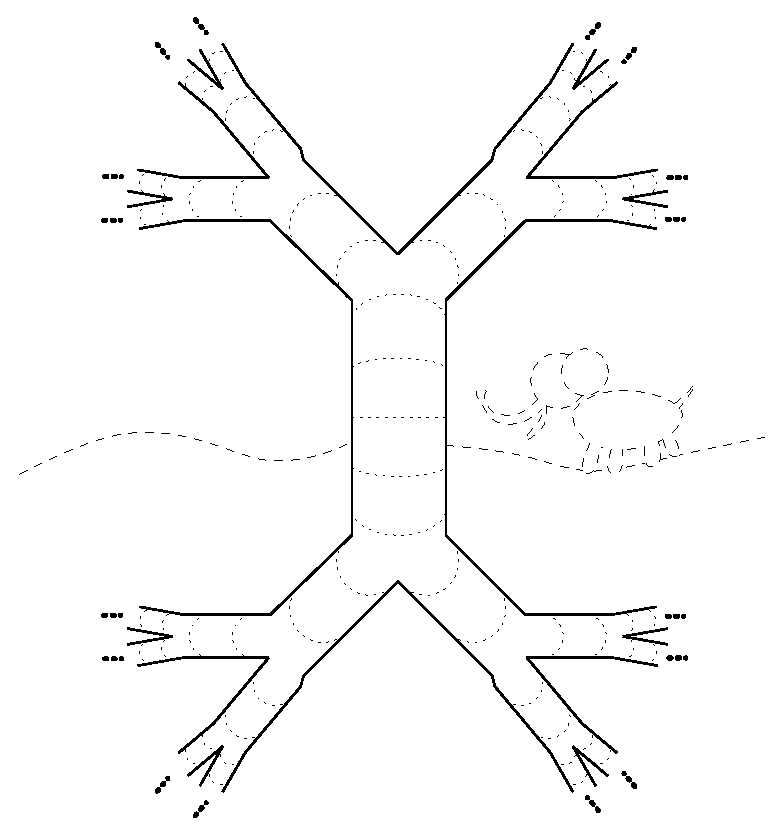
\includegraphics[width=100mm]{img/baobab.eps}
\caption{,,Baobab'', czyli oswojony do wewnątrz wielościan $X$~z~przykładu \ref{ex-o_baobabie}; rozważane w~tym przykładzie odwzorowanie $f\colon X\to X$~ma wiele wspólnego z~popularną legendą dotyczącą tego gatunku drzew.}\label{fig-baobab}
\end{figure}


%----------------------------------------------------------
%----------------------------------------------------------
%----------------------------------------------------------


\subsection{Potulność w~nieskończoności}
W~niniejszej sekcji przedstawiamy technikę dowodu twierdzenia o~punkcie lub końcu stałym, która wydaje się intuicyjna, ale ma raczej ograniczone zastosowanie. Jej istota zawiera się w~następującej obserwacji.

\begin{lem}\label{lem-ink_izo_na_hom}
Załóżmy, że $\F X$ jest \mbox{ANR-em} oraz włożenie $i\colon X\hookrightarrow \F X$ indukuje izomorfizm na grupach homologii. Wówczas homologie singularne przestrzeni $X$~są skończonego typu oraz zachodzi równość $\lambda(f)=\Ind(f)$.
\end{lem}
\begin{proof}
Ponieważ $\F X$ jest zwartym {ANR-em}, homologie tej przestrzeni są skończonego typu (patrz twierdzenie \ref{tw-westa}). Wobec tego przestrzeń $X$~również ma homologie~skończonego typu.

Niech $h_*\colon H_*(\F X)\to H_*(X)$ będzie izomorfizmem odwrotnym do izomorfizmu $H_*(i)\colon H_*(X)\to H_*(\F X)$. Zauważmy, że \begin{align*}H_*(i)\circ H_*(f)\circ h_*&=H_*(i\circ f)\circ h_*=H_*(\F f\circ i)\circ h_*\\&=H_*(\F f)\circ H_*(i)\circ h_*= H_*(\F f),\end{align*} zatem $\lambda\left(H_*(i)\circ H_*(f)\circ h_*\right)=\lambda(\F f)$. Z~drugiej strony \[\lambda(H_*(i)\circ H_*(f)\circ h_*)=\lambda(h_*\circ H_*(i)\circ H_*(f))=\lambda(H_*(f))=\lambda(f),\] co wynika z~lematu \ref{lem-1szy_lemat_o_liczbie_lefschetza}. Na podstawie~lematu \ref{lem-indeks-rowny-liczbie-lefschetza-uzwarcenia-freudenthala} ma miejsce równość $\lambda(\F f)=\Ind(f)$.\end{proof}

Istotnym przypadkiem, w~którym lemat \ref{lem-ink_izo_na_hom} ma zastosowanie, jest sytuacja, w~której $X$ jest przestrzenią potulną w nieskończoności. Jedna z~równoważnych definicji tej własności jest następująca. Mówimy, że przestrzeń $X$~będącą \mbox{ANR-em} jest \textit{potulna w nieskończoności}\footnote{ang. \textit{docile at infinity}}\index{przestrzenzzz topologiczna@przestrzeń topologiczna!potulna w nieskonzzzczonoszzzci@potulna w nieskończoności}\index{ANR!potulny w nieskonzzzczonoszzzci@potulny w nieskończoności}  \cite{Sher76}, o~ile dla każdego zwartego zbioru $A\subseteq X$ istnieje zwarty zbiór $A\subseteq B\subseteq X$ taki, że każda składowa spójności przestrzeni $X\smallsetminus B$ jest ściągalna w~$X\smallsetminus A$.

\begin{stw}\label{stw-pot_w_nsk_tw_lef}
Niech $X$ będzie potulnym w~nieskończoności \mbox{ANR-em}. Wówczas homologie singularne przestrzeni $X$~są skończonego typu oraz $\lambda(f)=\Ind(f)$.
\end{stw}
\begin{proof}
Przestrzeń $\F X$ jest \mbox{ANR-em} \cite[Theorem 4.2]{Sher76} oraz włożenie $X\hookrightarrow\F X$ jest homotopijną równoważnością \cite[Theorem 4.4]{Sher76}. Z~lematu \ref{lem-ink_izo_na_hom} otrzymujemy tezę.
\end{proof}

\begin{uw}
Stwierdzenie \ref{stw-pot_w_nsk_tw_lef} można otrzymać również jako wniosek z~twierdzenia \ref{tw-lefschetz_fpt_dla_reverse_tame}, gdyż uzwarcenie Freudenthala lokalnie zwartego, potulnego w~nieskończoności ANR-u jest $\mathcal{Z}$-uzwarceniem \cite[Theorem 4.4]{Sher76}, a~zatem taki ANR jest przestrzenią oswojoną do wewnątrz (patrz przykład \ref{przyklady-oswojonych-do-wewnatrz}).
\end{uw}

Ośrodkową, lokalnie zwartą przestrzeń metryczną $Y$ nazywamy \textit{APR-em}\footnote{ang. \textit{absolute proper retract}}\index{APR} \cite{Sher75}, jeżeli dla każdej ośrodkowej, lokalnie zwartej przestrzeni metrycznej $Z$~i~każdego włożenia $j\colon Y\hookrightarrow Z$ na podzbiór domknięty $j(Y)\subseteq Z$~takiego, że funkcja $\E(j)\colon \E(Y)\to \E(Z)$~jest różnowartościowa, istnieje właściwa retrakcja $r\colon Z\to j(Y)$.

\begin{wn}
Jeśli $X$~jest \mbox{APR-em}, to $X\in\FPEP$.
\end{wn}
\begin{proof}
Każdy \mbox{APR} jest potulnym w~nieskończoności, ściągalnym \mbox{ANR-em} \cite[Theorem 4.5]{Sher76}. Jeżeli więc $X$~jest APR-em, to dla każdego właściwego odwzorowania $g\colon X\to X$ bez końców stałych zachodzi na podstawie stwierdzenia \ref{stw-pot_w_nsk_tw_lef} równość $\lambda(g)=\Ind(g)$. Ale $\lambda(g)=1$, gdyż przestrzeń $X$~jest ściągalna. Z~własności (III) indeksu punktów stałych otrzymujemy $\Fix(g)\not=\emptyset$. 
\end{proof}

Każdy ściągalny w~sposób właściwy ANR jest APR-em \cite[Theorem 4.1]{Sher75}. Otrzymujemy stąd następujący wniosek, który odpowiada na pytanie postawione w~problemie \ref{PROBLEM-sciagalny-ma-fpep} w~przypadku, gdy rozważana przestrzeń jest ściągalna w~sposób właściwy. (Nie daje on jednak pełnej odpowiedzi na wspomniane pytanie.)

\begin{wn}\label{wn-sciagalny_w_sp_wlasciwy_to_FPEP}
Jeśli $X$ jest ściągalnym w~sposób właściwy \mbox{ANR-em}, to $X\in\FPEP$.
\end{wn}



%----------------------------------------------------------
%----------------------------------------------------------
%----------------------------------------------------------



\subsection{Końce oswojone na zewnątrz}\label{subsec-fixed_ends_dla_osw_na_zewn}
Obok obowiązujących założeń o~przestrzeni $X$~oraz odwzorowaniu $f\colon X\to X$ \textbf{do końca sekcji \ref{subsec-fixed_ends_dla_osw_na_zewn} zakładamy, że $X$~jest oswojonym na zewnątrz \mbox{ANR-em}.} Dowód twierdzenia Lefschetza o punkcie lub końcu stałym dla tego typu przestrzeni jest nieco bardziej złożony niż rozumowania przedstawione w~poprzednich sekcjach i~składa się z~kilku lematów.

\begin{lem}\label{lem-forward_tame_ma_sk_wiele_koncow}
Zbiór $\E(X)$ jest skończony.
\end{lem}
\begin{proof}
Ponieważ przestrzeń $X$~jest oswojona na zewnątrz, istnieje taki domknięty, koograniczony podzbiór $V\subseteq X$, o~dopełnieniu $C=X\smallsetminus V$, że włożenie $h_0\colon V\times\{0\}\hookrightarrow X$ rozszerza się do właściwego odwzorowania \mbox{$h\colon V\times [0,\infty)\to X$}.

Przypuśćmy, że $X$~ma nieskończenie wiele końców. Na podstawie lematu \ref{lem-malo_nieogr_skl} istnieje składowa spójności $S$~zbioru $V$~taka, że $\varepsilon(C)=S$ dla nieskończenie wielu końców $\varepsilon\in \E(X)$. Ustalmy dwa różne końce $\varepsilon_0,\varepsilon_1\in\E(X)$ o tej własności. Istnieje zbiór zwarty $D\subseteq X$ taki, że $\varepsilon_0(D)\not=\varepsilon_1(D)$. 

Ponieważ odwzorowanie $h$ jest właściwe, istnieje $t\in [0,\infty)$ o~tej własności, że $h(V,t)\cap D=\emptyset$. Funkcja $h_t=h(\cdot,t)$ jest homotopijna w~sposób właściwy odwzorowaniu $h_0$, zatem $\E(h_t)(\varepsilon_i)=\E(h_0)(\varepsilon_i)=\varepsilon_i$, gdzie $i=0,1$. Ale to oznacza, że 
\begin{equation}\label{lem-forward_tame_ma_sk_wiele_koncow-eq1} 
h_t\left(\varepsilon_i\left(h_t^{-1}(D)\right)\right)\subseteq \E(h_t)(\varepsilon_i)(D)=\varepsilon_i(D).
\end{equation}
Zachodzą inkluzje $\emptyset\not=\varepsilon_i\bigl(C\cup h_t^{-1}(D)\bigr)\subseteq \varepsilon_i(C)=S$ oraz $\varepsilon_i\bigl(C\cup h_t^{-1}(D)\bigr)\subseteq \varepsilon_i\bigl(h_t^{-1}(D)\bigr)$, zatem \begin{equation}\label{lem-forward_tame_ma_sk_wiele_koncow-eq2}\emptyset\not=\varepsilon_i\left(C\cup h_t^{-1}(D)\right)\subseteq \varepsilon_i\left(h_t^{-1}(D)\right)\cap S.\end{equation} Zestawiając~(\ref{lem-forward_tame_ma_sk_wiele_koncow-eq1})~i~(\ref{lem-forward_tame_ma_sk_wiele_koncow-eq2})~otrzymujemy $h_t(S)\cap\varepsilon_i(D)\not=\emptyset$ dla $i=0,1$. To jednak jest niemożliwe, gdyż $\varepsilon_0(D),\varepsilon_1(D)$ są różnymi składowymi spójności zbioru $X\smallsetminus D$, a~zbiór $h_t(S)$ jest spójny (jako obraz spójnego zbioru $S$) oraz $h_t(S)\cap D=\emptyset$.
\end{proof}

Dowód poniższego lematu jest wzorowany na dowodzie analogicznego wyniku dotyczącego uzwarcenia jednopunktowego, podanym w~książce Hughesa i~Ranickiego \cite{Hughes96}.  

\begin{lem}[por. {\cite[Proposition 7.11]{Hughes96}}]\label{lem-osw_nap_ANR}
Uzwarcenie Freudenthala $\F X$ przestrzeni $X$~jest \mbox{ANR-em}.
\end{lem}
\begin{proof}
Na podstawie~lematu \ref{lem-uzwarcenie_jest_metryczne} przestrzeń $\F X$ jest metryzowalna.

Wobec lematu \ref{lem-forward_tame_ma_sk_wiele_koncow} zbiór $\E(X)$ jest skończony. Oznaczmy jego elementy przez $\varepsilon_1,\ldots,\varepsilon_n$. Niech $V$ będzie domkniętym, koograniczonym podzbiorem $X$, dla którego istnieje właściwe odwzorowanie $q:V\times [0,\infty)\to X$ będące rozszerzeniem włożenia $V\times \{0\}\hookrightarrow X$; zbiór taki istnieje, gdyż przestrzeń $X$~jest oswojona na zewnątrz.

Przypuśćmy, że $\F X$ jest zanurzone jako domknięty podzbiór w~pewnej przestrzeni metrycznej $Z$. Ponieważ (będący \mbox{ANR-em}) zbiór $X=\F X\smallsetminus \E(X)$ jest domknięty w~$Z\smallsetminus \E(X)$, możemy znaleźć jego otwarte otoczenie $N$ w~$Z\smallsetminus \E(X)$ oraz retrakcję $r\colon N\to X$.

Niech $\{U_i\}_{i=1}^n$ będzie rodziną otwartych podzbiorów przestrzeni $Z$~o~następujących własnościach: $\varepsilon_i\in U_i$, $\overline{U_i}^Z\cap \overline{X\smallsetminus V}^Z=\emptyset$ oraz $\overline{U_i}^Z\cap\overline{U_j}^Z=\emptyset$ dla wszystkich $i,j=1,\ldots,n$, $i\not=j$; rodzina taka istnieje, gdyż przestrzeń $Z$~spełnia aksjomat oddzielania $\mathrm{T}_3$ (por.~\cite[Twierdzenie 1.5.5]{Engelking75}). Ustalmy zbiór $O\subseteq Z\smallsetminus \E(X)$ otwarty w~$Z\smallsetminus\E(X)$ i~taki, że \[X\subseteq O\subseteq \overline{O}^{Z\smallsetminus \E(X)}\subseteq N\] oraz \[\left(\overline{U_i}^Z\smallsetminus r^{-1}(\operatorname{Int}_X(V))\right)\cap \overline{O}^Z=\{\varepsilon_i\}\] dla wszystkich $i=1,\ldots,n$. Intuicyjnie, ,,w~pobliżu'' końców zbiór $\overline{O}^{Z\smallsetminus \E(X)}$~powinien zawierać się w~zbiorze $r^{-1}(\Int_X(V))$, otwartym w~przestrzeni $Z\smallsetminus \E(X)$.

Na podstawie~lematu Urysohna istnieje ciągła funkcja \[\rho:\left(\bigcup_{i=1}^n \overline{U_i}^Z\cup \overline{O}^Z\right)\smallsetminus \E(X)\to [0,\infty]\] taka, że $\rho^{-1}(0)=\overline{O}^Z$ oraz \[\rho^{-1}(\infty)=\left(\bigcup_{i=1}^n \overline{U_i}^Z\right)\smallsetminus \left(r^{-1}(\operatorname{Int}_X(V))\cup \E(X)\right).\] Odwzorowanie $\hat{r}:\left(\bigcup_{i=1}^{n} U_i\right)\cup O\to \F X$ określone dla $x\in\left(\bigcup_{i=1}^{n} U_i\right)\cup O$ wzorem
\[\hat{r}(x)=\begin{cases}\varepsilon_i, & \text{jeżeli } x\in \overline{U_i}^Z\smallsetminus r^{-1}(\operatorname{Int}_X(V)),\\
q(r(x),\rho(x)), & \text{jeżeli } x\in r^{-1}(V),\\
r(x), & \text{jeżeli } x\in \overline{O}^Z\smallsetminus r^{-1}(V).
\end{cases}\]
jest ciągłą retrakcją.
\end{proof}

\begin{lem}\label{lem-ANR_osw_nap_izo_hom}
Zachodzi naturalny izomorfizm $H^{\lf}_*(X)\cong H_*(\F X,\E(X))$.
\end{lem}
\begin{proof}
Zgodnie z~lematem \ref{lem-osw_nap_ANR} przestrzeń $\F X$ jest \mbox{ANR-em}. Wobec stwierdzenia \ref{stw-domkniety_podzbior_anr_jest_korozwloknieniem} włożenie skończonego zbioru dyskretnego $\E(X)$ w~przestrzeń $\F X$ jest korozwłóknieniem. Na podstawie stwierdzenia \ref{stw-homologie_ilorazu} istnieje naturalny izomorfizm \[H_*(\F X,\E(X))\cong H_*\left(\F X\big /\E(X),e\right),\] gdzie $e$~jest punktem odpowiadającym obrazowi zbioru $\E(X)$ w~przestrzeni ilorazowej $\F X\big/\E(X)$. Ale przestrzeń $\F X\big/\E(X)$ jest homeomorficzna uzwarceniu jednopunktowemu $X$ (lemat \ref{lem-iloraz_homeomorficzny_jednopunktowemu}). Zastosowanie twierdzenia \ref{tw-ranicki-hughes-izo-miedzy-homologiami-lf-a-uzwarcenia} kończy dowód.
\end{proof}

\begin{tw}\label{tw-lefschetz_fpt_dla_forward_tame}
Niech $X$~będzie oswojonym na zewnątrz \mbox{ANR-em}. Wówczas lokalnie skończone homologie $H_*^\lf(X)$ są skończonego typu i~jeśli $\lambda\left(H_*^\lf(f)\right)\not=0$, to $\Fix(f)\not=\emptyset$. Ponadto, jeżeli homomorfizm $H_*(f)$ jest dopuszczalny, to $\Lambda(f)=\lambda\left(H_*^\lf(f)\right)$.
\end{tw}
\begin{proof}
Wobec twierdzenia \ref{tw-ranicki-hughes-izo-miedzy-homologiami-lf-a-uzwarcenia} lokalnie skończone homologie $H_*^{\lf}(X)$ są izomorficzne zredukowanym homologiom singularnym zwartego \mbox{ANR-u}, a~zatem są skończenie generowane na podstawie twierdzenia \ref{tw-westa}. Liczba $\lambda\left(H_*^\lf(f)\right)$ jest więc dobrze określona. Jeżeli homomorfizm $H_*(f)$ jest dopuszczalny, to $\Lambda(f)=\lambda\left(H_*^\lf(f)\right)$ na podstawie lematu \ref{lem-rownosc_liczb_lefschetza_lf_i_zwyklej}

Wykażemy, że jeśli $\lambda\left(H_*^\lf(f)\right)\not=0$, to $\Fix(f)\not=\emptyset$. Na podstawie lematu \ref{lem-ANR_osw_nap_izo_hom} zachodzi równość: \[\lambda\left(H_*^\lf(f)\right)=\lambda\big(H_*(\F f, \E(X))\big).\] Z lematu \ref{lem-osw_nap_ANR} wiemy, że $\F X$ jest \mbox{ANR-em}. Zgodnie z~twierdzeniem \ref{tw-lefschetza_o_punkcie_stalym} odwzorowanie $\F f$ ma punkt stały w~zbiorze $\overline{\F X\smallsetminus \E(X)}=\F X$. Ale $\FixEnd(f)=\emptyset$, więc $\Fix(\F f)\cap \E(X)=\emptyset$, stąd $\F f$ ma punkt stały w~zbiorze $\F X\smallsetminus \E(X)=X$. Ponieważ $\F f\big|_X=f$, jest on również punktem stałym $f$.
\end{proof}

W~przypadku oswojonych na zewnątrz ANR-ów nie jest znana odpowiedź na pytanie o~związek liczby Lefschetza z~indeksem punktów stałych, postawione w~problemie \ref{PROBLEM-twierdzenie-o-indeksie}.

Poniżej podajemy przykład oswojonego na zewnątrz, lokalnie zwartego wielościanu $X$~oraz właściwego odwzorowania bez końców stałych $f\colon X\to X$ o~tej własności, że liczba $\lambda\left(H_*^\lf(f)\right)$ jest dobrze określona, ale homomorfizmy $H_*(f)$, $H_*^\infty(f)$ nie są dopuszczalne.

\begin{ex}\label{ex-osw_do_wew_bez_l_lef}
Dla każdej liczby naturalnej $n$~niech \[A_n=\left\{(x,y)\in\mathbb{R}^2:x^2+(y-2n)^2=1\right\}.\] Za przestrzeń $X$~przyjmijmy (przedstawiony na rysunku \ref{fig-organy}) zbiór
\[X=\bigcup_{n\in\mN}A_n\times \bigl( (-\infty,-n]\cup [n,\infty) \bigr),\] 
z~topologią indukowaną z~$\mathbb{R}^3$, zaś $f\colon X\to X$ niech będzie dla $(x,y,z)\in X$ dane wzorem $f(x,y,z)=(x,y,-z)$. Oczywiście odwzorowanie $f$~jest właściwe i~$\FixEnd(f)=\emptyset$. Nietrudno również spostrzec, że $X$~jest oswojonym na zewnątrz wielościanem, wobec czego liczba $\lambda^{\lf}(f)$ jest dobrze określona na podstawie twierdzenia \ref{tw-lefschetz_fpt_dla_forward_tame}. Jednak homomorfizmy $H_*(f)$, $H^\infty_*(f)$ nie są, jak łatwo zauważyć, dopuszczalne.
\end{ex}

\begin{figure}[h]
\centering
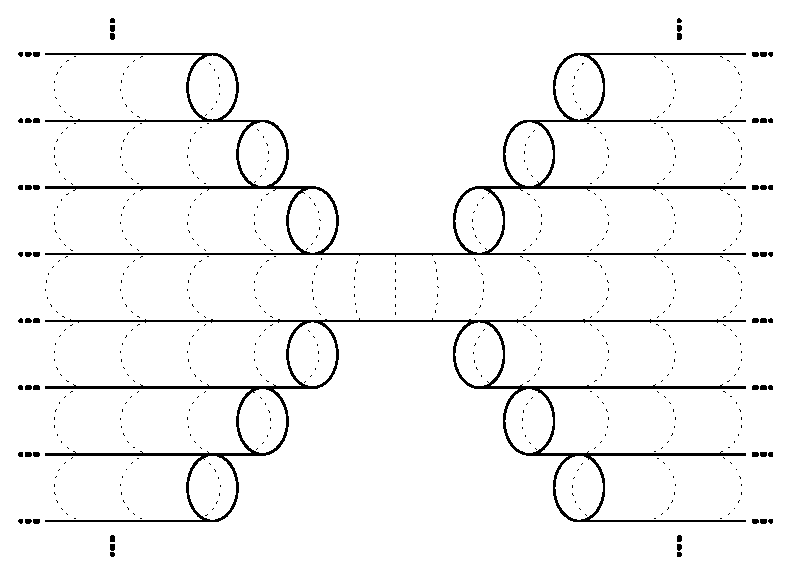
\includegraphics[width=100mm]{img/organki.eps}
\caption{,,Piszczałki organowe'', czyli oswojony na zewnątrz wielościan $X$~z~przykładu \ref{ex-osw_do_wew_bez_l_lef}.}\label{fig-organy}
\end{figure}




%----------------------------------------------------------
%----------------------------------------------------------
%----------------------------------------------------------




\section{Kombinatoryczne twierdzenia o~punkcie lub końcu stałym}\label{sec-komb_twi_o_punkcie_stalym}

W~niniejszym podrozdziale przenosimy podstawowe definicje związane z~końcami stałymi z~przypadku ciągłego na teorioporządkowy oraz symplicjalny, a~także rozwiązujemy dyskretne odpowiedniki problemów \ref{PROBLEM-twierdzenie-lefschetza-o-punkcie-lub-koncu-stalym}, \ref{PROBLEM-twierdzenie-o-indeksie}, \ref{PROBLEM-sciagalny-ma-fpep}. Otrzymujemy twierdzenia typu Lefschetza o~punkcie lub końcu stałym dla odwzorowań zachowujących porządek oraz odwzorowań symplicjalnych. Badamy ponadto związki własności punktu lub końca stałego z~pojęciem (ko)rozbieralności oraz z~operacją iloczynu kartezjańskiego zbiorów częściowo uporządkowanych.

\subsection{Definicje}
Zachowujące porządek odwzorowanie  $f\colon P\to Q$ nazywamy \textit{właściwym}\index{odwzorowanie!zachowujazzzce porzazzzdek@zachowujące porządek!wlzzzaszzzciwe@właściwe}, jeśli dla każdego $q\in Q$ zbiór $f^{-1}(q)$ jest skończony.

\textit{Końcem}\index{koniec!czezzzszzzciowego porzazzzdku@częściowego porządku} lokalnie skończonego częściowego porządku $P$~nazywamy funkcję \[\varepsilon\colon \{A\subseteq P:A\text{ jest skończony}\}\to 2^P\] spełniającą następujące warunki:
\begin{compactitem}
\item[---] jeżeli $A\subseteq B$ są skończonymi zbiorami zawartymi w~$P$, to $\varepsilon(B)\subseteq \varepsilon(A)$;
\item[---] dla każdego skończonego zbioru $A\subseteq P$ zbiór $\varepsilon(A)$ jest nieskończoną składową spójności częściowego porządku $P\smallsetminus A$.
\end{compactitem}
Zbiór końców porządku $P$~oznaczamy symbolem $\E(P)$.\nomenclature[6aa]{$\E$}{zb. koncow porzadku XXX do zbioru koncow zwyklego dopisz drugi numer strony}\index{zbiozzzr@zbiór!konzzzcozzzw@końców!czezzzszzzciowego porzazzzdku@częściowego porządku}

Jeśli $f\colon P\to Q$ jest właściwym odwzorowaniem zachowującym porządek między lokalnie skończonymi częściowymi porządkami, to możemy zadać odwzorowanie $\E(f)\colon \E(P)\to \E(Q)$ w~następujący sposób. Dla $\varepsilon\in \E(P)$ i~skończonego zbioru $A\subseteq Q$ niech $\E(f)(\varepsilon)(A)$ będzie jedyną spójną składową zbioru $Q\smallsetminus A$ taką, że \[f\left(\varepsilon\left(f^{-1}(A)\right)\right)\subseteq \E(f)(\varepsilon)(A).\] Przyporządkowanie $\E$ jest funktorialne.

Analogicznie jak w~przypadku ciągłych odwzorowań definiujemy \textit{koniec stały}\index{koniec!stalzzzy odwzorowania@stały odwzorowania!zachowujazzzcego porzazzzdek@zachowującego porządek} właściwego, zachowującego porządek odwzorowania $f\colon P\to P$ lokalnie skończonego częściowego porządku $P$~w~siebie, zbiór końców stałych $\FixEnd(f)$\nomenclature[3ba]{$\FixEnd(f)$}{wersja porzadkowa XXX}\index{zbiozzzr@zbiór!konzzzcozzzw stalzzzych odwzorowania@końców stałych odwzorowania!zachowujazzzcego porzazzzdek@zachowującego porządek} takiego odwzorowania oraz \textit{własność punktu lub końca stałego}\index{wlzzzasnoszzzczzz@własność!punktu lub konzzzca stalzzzego@punktu lub końca stałego!czezzzsciowego porzazzzdku@częściowego porządku}\index{czezzzszzzciowy porzazzzdek@częściowy porządek!ma wlzzzasnoszzzc@ma własność!punktu lub konzzzca stalzzzego@punktu lub końca stałego} ($\FPEP$)\nomenclature[3la]{$\FPEP$}{teorioporzadkowy XXX} ze względu na właściwe, zachowujące porządek przekształcenia. Dla lokalnie skończonego częściowego porządku $P$~i~właściwego odwzorowania $f\colon P\to P$ bez końców stałych definiujemy \textit{zbiór przestawiający końce}\index{zbiozzzr@zbiór!przestawiajazzzcy konzzzce@przestawiający końce!w czezzzsciowym porzazzzdku@w częściowym porządku} jako taki skończony zbiór $D\subseteq P$, że $f(\varepsilon(D))\cap \varepsilon(D)=\emptyset$ dla każdego końca $\varepsilon\in\E(X)$. Jeżeli porządek $P$~jest spójny, to zbiór taki istnieje, a~ponadto założyć o~nim można, że $P\smallsetminus D$ ma jedynie nieskończone składowe spójności. Faktów tych dowodzimy podobnie jak w~przypadku ciągłym.

Przez \textit{koniec}\index{koniec!kompleksu symplicjalnego} lokalnie skończonego kompleksu symplicjalnego $K$~rozumiemy koniec częściowego porządku $\mP(K)$; piszemy $\E(K)=\E(\mP(K))$\index{zbiozzzr@zbiór!konzzzcozzzw@końców!kompleksu symplicjalnego}. Odwzorowanie symplicjalne $\varphi\colon K\to L$ nazywamy \textit{właściwym}\index{odwzorowanie!symplicjalne!wlzzzaszzzciwe@właściwe}, o~ile funkcja zachowująca porządek $\mP(\varphi)\colon \mP(K)\to\mP(L)$ jest właściwa, lub równoważnie, o~ile realizacja geometryczna $|\varphi|\colon |K|\to |L|$ jest właściwym odwzorowaniem. Przyjmujemy oznaczenie $\E(\varphi)=\E(\mP(\varphi))$. Nietrudno jest wskazać naturalną bijekcję $\xi_K\colon \E(\mP(K))\to \E(|K|)$.

Jeśli $K$~jest lokalnie skończonym kompleksem symplicjalnym, to mówimy, że $K$~ma \textit{własność sympleksu lub końca stałego}\index{wlzzzasnoszzzczzz@własność!sympleksu lub konzzzca stalzzzego@sympleksu lub końca stałego}\index{kompleks symplicjalny!ma wlzzzasnoszzzc@ma własność!sympleksu lub konzzzca stalzzzego@sympleksu lub końca stałego} i~piszemy $K\in\FSEP$\nomenclature[3j]{$K\in\FSEP$}{lokalnie skończony kompleks symplicjalny $K$~ma własność sympleksu lub końca stałego}, o~ile dla każdego właściwego odwzorowania symplicjalnego $\varphi\colon K\to K$ istnieje sympleks stały lub \textit{koniec stały}\index{koniec!stalzzzy odwzorowania@stały odwzorowania!symplicjalnego}, tj.~taki koniec $\varepsilon\in \E(K)$, że $\E(\varphi)(\varepsilon)=\varepsilon$.

Oczywiście istnienie sympleksu stałego odwzorowania symplicjalnego implikuje istnienie punktu stałego jego realizacji geometrycznej, zaś każdy koniec stały odwzorowania symplicjalnego można utożsamiać (poprzez bijekcję $\xi_K$) z~końcem stałym realizacji geometrycznej tego odwzorowania.

Własność sympleksu lub końca stałego jest równoważna własności punktu lub końca stałego stowarzyszonego częściowego porządku.

\begin{stw}[por.~{\cite[Proposition 6.3.15]{Schroder03}}]\label{stw-simplicial_fpep_wtw_order_theoretic}
Jeżeli $K$~jest lokalnie skończonym kompleksem symplicjalnym, to $K\in\FSEP$ wtedy i~tylko wtedy, gdy $\mP(K)\in\FPEP$.
\end{stw}
\begin{proof}
Ustalmy lokalnie skończony kompleks symplicjalny $K$. 

Załóżmy, że $\mP(K)\in\FPEP$; niech $\varphi\colon K\to K$ będzie właściwym odwzorowaniem symplicjalnym bez końców stałych. Wówczas $\FixEnd(\mP(\varphi))=\emptyset$, więc $\Fix(\mP(\varphi))\not=\emptyset$, co oznacza, że istnieje sympleks $\sigma$~kompleksu $K$~taki, że $\varphi(\sigma)=\sigma$. Wobec tego $K\in\FSEP$.

Załóżmy teraz, że $K\in\FSEP$ i~ustalmy właściwe, zachowujące porządek odwzorowanie $f\colon \mP(K)\to \mP(K)$ bez końców stałych. Dla każdego wierzchołka $v$~kompleksu $K$~wybierzmy dowolny element $g_v\in f(\{v\})$. Określmy funkcję $g\colon \mP(K)\to \mP(K)$, dla $\sigma\in \mP(K)$ przyjmując $g(\sigma)=\bigcup_{v\in\sigma}\{g_v\}$. Oczywiście $g$~zachowuje porządek. Nietrudno również sprawdzić (por.~\cite[Lemma 6.3.14]{Schroder03}), że odwzorowanie $\gamma\colon K\to K$ zadane na wierzchołkach $v\in K$ wzorem $\gamma(v)=g_v$ jest symplicjalne oraz $\mP(\gamma)=g$. Dla każdego sympleksu $\sigma\in \mP(K)$ i~każdego wierzchołka $v\in\sigma$ mamy $f(\sigma)\supseteq f(\{v\})\supseteq \{g_v\}= g(\{v\})$, więc $f(\sigma)\supseteq\bigcup_{v\in \sigma} g(\{v\})=g(\sigma)$. Jak łatwo zauważyć, wynika stąd, że $\E(g)=\E(f)$, czyli w~szczególności $\FixEnd(g)=\FixEnd(f)=\emptyset$. Ponieważ $g=\mP(\gamma)$, odwzorowanie $\gamma$~nie ma końców stałych, a~zatem istnieje sympleks stały $\sigma$~tego odwzorowania. Ale $f(\sigma)\supseteq g(\sigma)=\sigma$, więc na podstawie twierdzenia Abiana-Browna \ref{tw-abiana_browna} funkcja $f$~ma punkt stały, co kończy dowód stwierdzenia.
\end{proof}



%--------------------------------------------------------------------
%--------------------------------------------------------------------
%--------------------------------------------------------------------



\subsection{Odległość w~częściowym porządku}
Bieżąca sekcja poświęcona jest pomocniczemu pojęciu odległości między elementami częściowego porządku, które wykorzystane zostanie w~dalszej części rozdziału.

Jeżeli $p,q$ są elementami częściowego porządku $P$, to przez $d_P(p,q)$\nomenclature[4k]{$d_P(p,q)$}{odległość między elementami $p, q$~częściowego porządku $P$} oznaczamy \textit{odległość}\index{odleglzzzoszzzczzz w czezzzszzzciowym porzazzzdku@odległość w~częściowym porządku} $p$~od~$q$~w~zbiorze $P$, z~definicji równą minimalnej długości ścieżki prowadzącej z~$p$~do $q$~w~grafie porównywalności $\Comp(P)$, o~ile ścieżka taka istnieje; w~przeciwnym wypadku przyjmujemy $d_P(p,q)=\infty$. Dla $p\in P$ oraz $A\subseteq P$ niech $d_P(p,A)=\min\{d_P(p,q):q\in A\}$.\nomenclature[4l]{$d_P(p,A)$}{odległość punktu $p$~od zbioru $A$~w~częściowym porządku $P$}

Jeśli $f\colon P\to Q$ jest zachowującym porządek odwzorowaniem, to dla każdej ścieżki $(p_0,\ldots,p_n)$ w~$\Comp(P)$ ciąg $\big(f(p_0),\ldots,f(p_n)\big)$ jest ścieżką w~$\Comp(Q)$, zatem $d_Q(f(p),f(q))\leq d_P(p,q)$ dla wszystkich $p,q\in P$.

Dla częściowego porządku $P$, elementu $p\in P$ oraz liczby $n\in \mN$ przyjmujemy oznaczenie \[B_P(p,n)=\{q\in P:d_P(p,q)\leq n\}.\]\nomenclature[4m]{$B_P(p,n)$}{domknięta kula o~środku $p$~i~promieniu~$n$~w~zbiorze częściowo uporządkowanym $P$} Ponadto, jeśli $F\subseteq P$, to definiujemy zbiór \[B_P(F,n)=\bigcup_{p\in F}B_P(p,n)=\{q\in P:d_P(q,F)\leq n\}.\]\nomenclature[4n]{$B_P(A,n)$}{domknięta otoczka zbioru $A$~o~promieniu~$n$~w~zbiorze częściowo uporządkowanym $P$}Nietrudno spostrzec, że jeśli porządek $P$~jest lokalnie skończony, to dla każdego skończonego podzbioru $F\subseteq P$ oraz każdego $n\in\mN$~zbiór $B_P(F,n)$ jest skończony.

\begin{lem}\label{lem-odleglosc_miedzy_skladowymi_po_nadmuchaniu_srodka}
Niech $P$~będzie spójnym częściowym porządkiem, $F\subseteq P$ jego skończonym podzbiorem, $S\subseteq P$ składową spójności zbioru $P\smallsetminus F$ oraz niech $k\in\mN$. Wówczas $d_P(p,q)> k$ dla wszystkich $p\in S$, $q\in P\smallsetminus \left(S\cup B_P(F,k)\right)$.
\end{lem}
\begin{proof}
Zauważmy, że dla wszystkich elementów $p\in S$ oraz $q\in P\smallsetminus (S\cup F)$ każda ścieżka prosta w~grafie porównywalności $\Comp(P)$ prowadząca z~$p$~do $q$~zawiera element zbioru $F$; zachodzi zatem nierówność \[d_P(p,q)\geq d_P(p,F)+d_P(q,F).\] Wobec tego dla $p\in S$ oraz $q\in P\smallsetminus \left(S\cup B_P(F,k)\right)$ mamy \[d_P(p,q)\geq d_P(p,F)+d_P(q,F)\geq d_P(p,F)+k+1>k.\qedhere\] 
\end{proof}

\begin{lem}\label{lem-bliskie_funkcje_to_samo_na_koncach}
Niech $P,Q$~będą lokalnie skończonymi częściowymi porządkami, zaś $f,g\colon P\to Q$ właściwymi odwzorowaniami zachowującymi porządek. Jeżeli istnieje $k\in\mN$ takie, że dla każdego $p\in P$ zachodzi nierówność $d_Q(f(p),g(p))\leq k$, to $\E(f)=\E(g)$.
\end{lem}
\begin{proof}
Załóżmy, że istnieje liczba $k\in \mN$ taka, że $d_Q(f(p),g(p))\leq k$ dla każdego $p\in P$. Aby udowodnić równość $\E(f)=\E(g)$ wystarczy wykazać, że dla każdego końca $\varepsilon\in \E(P)$ i~każdego skończonego podzbioru $F\subseteq Q$ mamy 
\mbox{$\E(f)(\varepsilon)(F)\cap \E(g)(\varepsilon)(F)\not=\emptyset$}. Ustalmy zatem koniec $\varepsilon\in \E(P)$ oraz skończony zbiór $F\subseteq Q$. 

Zauważmy, że \[g^{-1}(F)\subseteq f^{-1}\big(B_Q(F,k)\big)\supseteq f^{-1}(F),\] więc \[\varepsilon\big(g^{-1}(F)\big)\supseteq \varepsilon\left(f^{-1}\big(B_Q(F,k)\big)\right)\subseteq \varepsilon\big(f^{-1}(F)\big).\]
Ustalmy $p\in \varepsilon\bigl(f^{-1}\big(B_Q(F,k)\big)\bigr)$; mamy \begin{align*}f(p)&\in f\left( \varepsilon\big(f^{-1}(F)\big)\right)\subseteq \E(f)(\varepsilon)(F),\\ g(p)&\in  g\left(\varepsilon\big(g^{-1}(F)\big)\right)\subseteq \E(g)(\varepsilon)(F)\end{align*} oraz $d_Q(f(p),F)>k$. Ale $d_Q(f(p),g(p))<k$, więc $g(p)\in \E(f)(\varepsilon)(F)$ na podstawie lematu \ref{lem-odleglosc_miedzy_skladowymi_po_nadmuchaniu_srodka}. Wobec tego $\E(f)(\varepsilon)(F)\cap \E(g)(\varepsilon)(F)\not=\emptyset$.
\end{proof}


%-------------------------------------------------------------------
%-------------------------------------------------------------------
%-------------------------------------------------------------------




\subsection{Kombinatoryczne twierdzenie typu Lefschetza o~punkcie lub końcu stałym}\label{subsec-komb_twi_lefschetza}
\textbf{Odtąd, aż do końca sekcji \ref{subsec-komb_twi_lefschetza}, zakładamy, że $P$~jest spójnym, lokalnie skończonym częściowym porządkiem, zaś $f\colon P\to P$ jest właściwym odwzorowaniem zachowującym porządek bez końców stałych.}

Jeśli $h\colon A\to A$ jest funkcją określoną na pewnym zbiorze $A$, to mówimy, że $a\in A$ jest jej \textit{punktem periodycznym}\index{punkt!periodyczny}, o ile $h^m(a)=a$ dla pewnej liczby naturalnej $m\geq 1$. Jeżeli natomiast istnieje liczba naturalna $n$ taka, że $h^{n}(a)$ jest punktem periodycznym funkcji $h$, to $a$ nazywamy \textit{punktem ostatecznie periodycznym}\index{punkt!ostatecznie periodyczny} funkcji $h$.

\begin{lem}\label{lem-kazdy_punkt_ost_periodyczny}
Każdy element $p\in P$ jest punktem ostatecznie periodycznym odwzorowania~$f$. 
\end{lem}
\begin{proof}
Ustalmy element $p\in P$ i~przypuśćmy, że nie jest on punktem ostatecznie periodycznym funkcji $f$. Przyjmijmy oznaczenie $k=d_P(p,f(p))$; porządek $P$~jest spójny, więc $k<\infty$. Ponieważ $f$~zachowuje porządek, prawdziwa jest dla wszystkich $n\in\mN$ nierówność 
\begin{equation}d_P\left(f^n(p),f^{n+1}(p)\right)\leq k.\label{eq_lem-kazdy_punkt_1}\end{equation} Istnieje podzbiór $D\subseteq P$ przestawiający końce i~taki, że $P\smallsetminus D$ nie ma skończonych składowych spójności.  Ponieważ punkt $p$~nie jest ostatecznie periodyczny, a~zbiór $B_P(D,k)$~jest skończony, istnieje liczba $n_0\in\mN$ taka, że $f^n(p)\not\in B_P(D,k)$ dla wszystkich $n\geq n_0$. W~szczególności $f^{n_0}(p)\not\in D$, więc $f^{n_0}(p)\in \varepsilon(D)$ dla pewnego końca $\varepsilon\in\E(P)$. Ponieważ $D$~jest zbiorem przestawiającym końce, $f^{n_0+1}(p)\not\in \varepsilon(D)$, a~z~wyboru liczby $n_0$~element $f^{n_0+1}(p)\not\in B_P(D,k)$. Zatem $f^{n_0+1}(p)\in P\smallsetminus (\varepsilon(D)\cup B_P(D,k))$. Na podstawie lematu \ref{lem-odleglosc_miedzy_skladowymi_po_nadmuchaniu_srodka} zachodzi nierówność $d_P\left(f^{n_0+1}(p),f^{n_0}(p)\right)> k$, sprzeczna z~nierównością (\ref{eq_lem-kazdy_punkt_1}).
\end{proof}

\begin{lem}\label{lem-wsz_per_odw_aut}
Niech $Q$~będzie częściowym porządkiem, zaś $g\colon Q\to Q$ zachowującym porządek odwzorowaniem o~tej własności, że każdy element zbioru $Q$ jest punktem periodycznym funkcji~$g$. Wówczas $g$~jest automorfizmem częściowego porządku $Q$.
\end{lem}
\begin{proof}
Dowód lematu jest nietrudny; należy zauważyć, że odwzorowanie $g$~jest różnowartościowe i~,,na'', oraz że jeśli $g(p)\leq g(q)$ dla pewnych $p,q\in Q$, to również $p\leq q$. Dla przykładu udowodnimy tę ostatnią własność. 

Jeśli $p\leq q$, to $g^n(p)\leq g^n(q)$ dla każdej liczby $n\in\mN$. Ponieważ $p,q$ są punktami periodycznymi funkcji $g$, istnieją liczby naturalne $n_p,n_q$ takie, że $g^{n_p}(p)=p$ oraz $g^{n_q}(q)=q$, a~zatem: \[p=g^{n_p n_q}(p)\leq g^{n_p n_q}(q)=q.\qedhere\]
\end{proof}

Oznaczmy przez $P_\infty$~podzbiór częściowo uporządkowany zbioru $P$, którego elementami są wszystkie punkty periodyczne odwzorowania $f$. Oczywiście $f(P_\infty)\subseteq P_\infty$. Niech $f_\infty=f\big |_{P_\infty}\colon P_\infty\to P_\infty$. Na podstawie lematu \ref{lem-wsz_per_odw_aut} odwzorowanie to jest automorfizmem częściowego porządku $P_\infty$. Ponieważ \mbox{$\FixEnd(f)=\emptyset$}, jest oczywiste, że $\FixEnd(f_\infty)=\emptyset$.

Przypomnijmy, że z~definicji homologie częściowego porządku $Q$~są równe symplicjalnym homologiom stowarzyszonego z~nim kompleksu symplicjalnego $\mK(Q)$. Są to zatem homologie pewnego kompleksu łańcuchowego $C_*(Q)=\left(C_i(Q),\partial_i\right)_{i\in\mN}$ takiego, że dla każdego $i\in\mN$ bazą przestrzeni wektorowej $C_i(Q)$~jest zbiór łańcuchów długości $i$~zawartych w~$Q$. Jeżeli $A\subseteq Q$, to istnieje kompleks łańcuchowy $C_*(Q,A)=C_*(Q)\big/C_*(A)$ oraz $H_*(Q,A)=H_*(C_*(Q,A))$.

Jeżeli $Q$~jest częściowym porządkiem, $A\subseteq Q$, zaś $g\colon Q\to Q$ jest zachowującym porządek odwzorowaniem o~tej własności, że $g(A)\subseteq A$, to symbolem $g_{(Q,A)}\colon (Q,A)\to (Q,A)$ oznaczamy indukowane przez $g$~odwzorowanie par częściowych porządków.

\begin{lem}\label{lem-lambda_phi_nsk_rowna_lambda_phi}
Homomorfizm $H_*(f)$~jest dopuszczalny wtedy i~tylko wtedy, gdy homomorfizm $H_*(f_\infty)$ jest dopuszczalny. Ponadto zachodzi wówczas równość uogólnionych liczb Lefschetza: $\Lambda(f)=\Lambda(f_\infty)$.
\end{lem}
\begin{proof}
Istnieje przemienny diagram \[\xymatrix{\cdots \ar[r] & H_n(P_\infty)\ar[r]\ar^{H_n(f_\infty)}[d] & H_n(P)\ar^{H_n(f)}[d]\ar[r] & H_n(P,P_\infty)\ar[r]\ar^{H_n\left(f_{(P,P_\infty)}\right)}[d] & H_{n-1}(P_\infty)\ar[r]\ar^{H_{n-1}(f_\infty)}[d] & \cdots\\ \cdots\ar[r] & H_n(P_\infty)\ar[r] & H_n(P)\ar[r] & H_n(P,P_\infty)\ar[r] & H_{n-1}(P_\infty)\ar[r] & \cdots}\] o wierszach będących długimi ciągami dokładnymi pary $(P,P_\infty)$. Dla każdego elementu $\zeta\in H_*(P,P_\infty)$ istnieje łańcuch $z\in C_*(P)$ taki, że $\zeta$~jest klasą homologii elementu $z+C_*(P_\infty)\in C_*(P)\big/C_*(P_\infty)$, co zapisujemy przez $\zeta=[z+C_*(P_\infty)]$. Na podstawie lematu \ref{lem-kazdy_punkt_ost_periodyczny} istnieje liczba naturalna $n_z$~taka, że $C_*(f^{n_z})(z)\in C_*(P_\infty)$. Zatem \[H_*\left(f^{n_z}_{(P,P_\infty)}\right)(\zeta)=H_*\left(f^{n_z}_{(P,P_\infty)}\right)([z+C_*(P_\infty)])=[C_*(f^{n_z})(z)+C_*(P_\infty)]=0,\] czyli $\zeta$~należy do uogólnionego jądra: $\zeta\in N\bigl(H_*\bigl(f_{(P,P_\infty)}\bigr)\bigr)$. Wobec~dowolności wyboru $\zeta\in H_*(P,P_\infty)$~oznacza to, że homomorfizm $H_*\bigl(f_{(P,P_\infty)}\bigr)$ jest dopuszczalny oraz $\Lambda\bigl(H_*\bigl(f_{(P,P_\infty)}\bigr)\bigr)=0$. Z~lematu \ref{lem-2gi_lemat_o_liczbie_lefschetza} otrzymujemy równość $\Lambda(f)=\Lambda(f_\infty)$.
\end{proof}

Poniższe twierdzenie typu Lefschetza o~punkcie lub końcu stałym dla częściowych porządków jest uogólnieniem na lokalnie skończone częściowe porządki twierdzenia \ref{tw-baclawski-bjorner}.

\begin{tw}\label{tw-order-theoretic-fixed-point-or-end-theorem}
Jeśli homomorfizm $H_*(f)$ jest dopuszczalny, to zachodzi równość uogólnionej liczby Lefschetza odwzorowania $f$~oraz charakterystyki Eulera zbioru jego punktów stałych: $\Lambda(f)=\chi(\Fix(f))$.
\end{tw}
\begin{proof}
Załóżmy, że homomorfizm $H_*(f)$~jest dopuszczalny. Wybierzmy skończony podzbiór $D'\subseteq P_\infty$ taki, że $D'$~jest dla $f_\infty$ zbiorem przestawiającym końce. Ponieważ $f_\infty$ jest automorfizmem, możemy zakładać, że podzbiór $D'$ jest niezmienniczy ze względu na działanie $f_\infty$. Co więcej, możemy $D'$~rozszerzyć do niezmienniczego ze względu na $f_\infty$, skończonego podzbioru $D\subseteq P$ takiego, że zbiór $P_\infty\smallsetminus D$ nie ma skończonych składowych spójności.

Niech $A=P_\infty\smallsetminus D$. Wobec wyboru $D$ zbiór $A$ jest niezmienniczy ze względu na działanie automorfizmu $f_\infty$. Ponieważ zbiór $D=P_\infty\smallsetminus A$ jest skończony, kompleks łańcuchowy $C_*(P_\infty,A)$ oraz relatywne homologie $H_*(P_\infty,A)$ są skończonego typu. Istnieje przemienny diagram
\[
\xymatrix@R=30pt{\cdots\ar[r]& H_n(A)\ar[r]\ar[d]^{H_n\bigl(f\big |_A\bigr)}& H_n(P_\infty)\ar[r]\ar[d]^{H_n(f_\infty)} & H_n(P_\infty,A)\ar[r]\ar[d]^{H_n\bigl({f_\infty}_{(P_\infty,A)}\bigr)} & H_{n-1}(A)\ar[r]\ar[d]^{H_{n-1}\bigl(f\big |_A\bigr)} & \cdots\\
\cdots\ar[r]& H_n(A)\ar[r]& H_n(P_\infty)\ar[r] & H_n(P_\infty,A)\ar[r] & H_{n-1}(A)\ar[r] & \cdots}
\]
o~wierszach będących długimi ciągami dokładnymi pary $(P_\infty,A)$.
Homomorfizmy $H_*\bigl({f_\infty}_{(P_\infty,A)}\bigr)$ oraz $H_*(f_\infty)$ są dopuszczalne, co wynika odpowiednio z~faktu, że homologie $H_*(P_\infty,A)$ są skończonego typu i~z~lematu \ref{lem-lambda_phi_nsk_rowna_lambda_phi}. Na podstawie lematu \ref{lem-2gi_lemat_o_liczbie_lefschetza} homomorfizm $H_*\bigl(f\big |_A\bigr)$ jest dopuszczalny oraz \[\Lambda\bigl(f\big |_A\bigr)=\Lambda(f_\infty)-\Lambda\bigl({f_\infty}_{(P_\infty,A)}\bigr).\]

Niech $S_i$, $i=1,\ldots,k$, będą wszystkimi spójnymi składowymi zbioru $A$. Ponieważ $D$~jest dla $f_\infty$~zbiorem przestawiającym końce, dla wszystkich $i=1,\ldots,k$ mamy $f_\infty(S_i)\cap S_i=\emptyset$. Wobec teorioporządkowego odpowiednika lematu \ref{lem-permutowanie-skladowych-a-liczba-lefschetza} oznacza to, że $\Lambda\bigl(f\big |_A\bigr)=0$, czyli $\Lambda(f_\infty)=\Lambda\bigl({f_\infty}_{(P,A)}\bigr)$. Z~lematu \ref{lem-lambda_phi_nsk_rowna_lambda_phi} otrzymujemy równość $\Lambda(f)=\Lambda\bigl({f_\infty}_{(P,A)}\bigr)$.

Kompleks łańcuchowy $C_*(P_\infty,A)$ jest skończonego typu, wobec czego na podstawie~twierdzenia \ref{tw-lefschetza-hopfa} zachodzą równości \[\lambda\left(C_*\bigl({f_\infty}_{(P,A)}\bigr)\right)=\lambda\left(H_*\bigl({f_\infty}_{(P,A)}\bigr)\right)=\Lambda\bigl({f_\infty}_{(P,A)}\bigr).\] Bazę przestrzeni $C_*(P_\infty,A)$ tworzą skończone, liniowo uporządkowane podzbiory $P_\infty$~nie zawierające się w~$A$. Dla takiego bazowego podzbioru liniowo uporządkowanego $l\subseteq P_\infty$ oraz~skalara $\alpha\in\mathbb{Q}\smallsetminus \{0\}$ równość $C_*\bigl({f_\infty}_{(P,A)}\bigr)(l)=\alpha l$ ma miejsce wtedy i~tylko wtedy, gdy $f_\infty(l)=l$ oraz $\alpha=1$, gdyż $f_\infty$~jest odwzorowaniem zachowującym porządek. Ponieważ $\Fix(f_\infty)\subseteq P_\infty\smallsetminus A$, każdy bazowy podzbiór liniowo uporządkowany $l\subseteq P_\infty$~taki, że $C_*\bigl({f_\infty}_{(P,A)}\bigr)(l)=l$, jest również elementem bazowym przestrzeni liniowej $C_*(D)\subseteq C_*(P_\infty,A)$. Zachodzą  zatem równości \begin{align*}\lambda(C_*(f_\infty,A))&=\lambda\left(C_*\bigl(f\big |_D\bigr)\right)=\sum_{i=0}^{\infty}(-1)^i\tr\left(C_i\bigl(f\big|_D\bigr)\right)\\&=\sum_{i=0}^{\infty}(-1)^{i}\moc{\bigl\{\{q_0<\ldots<q_i\}\subseteq \Fix(f)\bigr\}} =\chi(\Fix(f)),\end{align*}
kończące dowód twierdzenia. 
\end{proof}

Oczywisty jest następujący wniosek.
\begin{wn}
Jeśli homomorfizm $H_*(f)$~jest dopuszczalny oraz~$\Lambda(f)\not=0$, to $\Fix(f)\not=\emptyset$.
\end{wn}

Prawdziwa jest także symplicjalna wersja twierdzenia \ref{tw-order-theoretic-fixed-point-or-end-theorem}, uogólniająca wniosek \ref{wn-baclawski-bjorner}.

\begin{wn}\label{wn-simplicial-fixed-point-or-end-theorem}
Niech $K$~będzie lokalnie skończonym kompleksem symplicjalnym, zaś $\varphi\colon K\to K$ właściwym odwzorowaniem symplicjalnym bez końców stałych. Jeśli homomorfizm $H_*(\varphi)$ jest dopuszczalny, to jego uogólniona liczba Lefschetza jest równa charakterystyce Eulera zbioru punktów stałych realizacji geometrycznej tego odwzorowania: $\Lambda(\varphi)=\chi(\Fix|\varphi|)$. 
\end{wn}
\begin{proof}
Oczywiście $\mP(\mK(\mP(K)))$ jest lokalnie skończonym częściowym porządkiem, zaś $\mP(\mK(\mP(\varphi)))$ jest właściwym odwzorowaniem zachowującym porządek bez końców stałych. Ponadto, jeśli homomorfizm $H_*(\varphi)$ jest dopuszczalny, to również homomorfizm $H_*(\mP(\mK(\mP(\varphi))))$ jest dopuszczalny i~zachodzi równość $\Lambda(\varphi)=\Lambda(\mP(\mK(\mP(\varphi))))$. Z~twierdzenia \ref{tw-order-theoretic-fixed-point-or-end-theorem} otrzymujemy: \[\Lambda(\varphi)=\chi(\Fix(\mP(\mK(\mP(\varphi)))))=\chi(\Fix(|\mK(\mP(\varphi))|))=\chi(\Fix(|\varphi|)).\qedhere\]
\end{proof}

Zauważmy, że funkcja z~przykładu \ref{ex-jacob-ladder} jest realizacją geometryczną odwzorowania symplicjalnego, co pokazuje, że w~powyższych wynikach nie można pominąć założenia o~dopuszczalności homomorfizmów indukowanych przez rozważane odwzorowania.

Poniższe twierdzenie wiąże uogólnioną liczbę Lefschetza odwzorowania symplicjalnego bez końców stałych z~indeksem punktów stałych jego realizacji geometrycznej.

\begin{tw}\label{tw-rownosc_indeksu_i_l_lefschetza_odwz_sympl}
Niech $K$~będzie lokalnie skończonym kompleksem symplicjalnym, zaś $\varphi\colon K\to K$ właściwym odwzorowaniem symplicjalnym bez końców stałych. Jeśli homomorfizm $H_*(\varphi)$ jest dopuszczalny, to uogólniona liczba Lefschetza odwzorowania symplicjalnego $\varphi$~jest równa indeksowi punktów stałych jego realizacji geometrycznej: $\Lambda(\varphi)=\Ind(|\varphi|)$.
\end{tw}
\begin{proof}
Na podstawie lematu \ref{lem-kazdy_punkt_ost_periodyczny} zastosowanego do odwzorowania $\mP(\varphi)\colon\mP(K)\to\mP(K)$ każdy wierzchołek kompleksu $K$~jest punktem ostatecznie periodycznym funkcji $\varphi$. Istnieje zatem wierzchołek $v_0\in K$ będący jej punktem periodycznym. Dla każdej liczby $n\in\mN$~niech $\widetilde{K}_n$~będzie pełnym podkompleksem $K$~rozpiętym na zbiorze wierzchołków \[V\bigl(\widetilde{K}_n\bigr)=\bigcup_{m\in\mN} \min\left(B_{\mP(K)}\bigl(\varphi^m(v_0),n\bigr)\right),\] zaś przez $K_n$~oznaczmy pełny podkompleks $K$~rozpięty na zbiorze wierzchołków \[V(K_n)=\bigcup_{m\in\mN}\left\{\varphi^m(w):w\in V\bigl(\widetilde{K}_n\bigr)\right\}.\] Kompleks $\widetilde{K}_n$ jest oczywiście skończony. Skończoność kompleksu $K_n$ wynika natomiast ze skończoności $\widetilde{K}_n$ oraz faktu, że każdy wierzchołek kompleksu $K$~jest ostatecznie periodyczny. Zauważmy, że $\bigcup_{n\in\mN}K_n=K$ oraz $|\varphi|(|K_n|)\subseteq |K_n|$ dla każdej liczby naturalnej $n$.

Zbiór $\Fix(|\varphi|)$ jest (na podstawie lematu \ref{lem-fixed_point_set_zwarty}) zwarty, a~zatem istnieją otwarty podzbiór $U\subseteq |K|$ oraz liczba $n_0\in\mN$ takie, że $\Fix(|\varphi|)\subseteq U\subseteq \left|K_{n_0}\right|$. Stosując kolejno lemat \ref{wlasnosc_viii}, aksjomat wycinania (I) oraz normalizacji (VII), otrzymujemy:
\[\Ind(|\varphi|)\!=\!\Ind\left(|\varphi|\big|_{U}\colon U\to |K_n|\right)\!=\!\Ind\left(|\varphi|\big|_{|K_n|}\colon |K_n|\to |K_n|\right)\!=\!\Lambda\left(|\varphi|\big|_{|K_n|}\right).\]
Ponieważ $\Fix\left(|\varphi|\big|_{|K_n|}\right)=\Fix(|\varphi|)$, na podstawie wniosku \ref{wn-simplicial-fixed-point-or-end-theorem} zachodzą równości:
\[\Lambda\left(|\varphi|\big|_{|K_n|}\right)=\chi\left(\Fix\left(|\varphi|\big|_{|K_n|}\right)\right)=\chi(\Fix(|\varphi|))=\Lambda(\varphi).\qedhere\]
\end{proof}



%-------------------------------------------------------------------
%-------------------------------------------------------------------
%-------------------------------------------------------------------



\subsection{(Ko)rozbieralność a~własność punktu lub końca stałego}\label{subsec-korozb_a_wl_FPEP}
Wskażemy związki między kombinatoryczną własnością punktu lub końca stałego a~pojęciem (ko)rozbieralności. Badanie ich jest naturalne, gdyż analogiczne powiązania okazały się niezwykle istotne dla teorii punktów stałych odwzorowań zachowujących porządek \cite{Schroder99,Schroder03,Schroder12}.

Mówimy, że para $(P,r)$, składająca się z~częściowego porządku $P$~oraz retrakcji $r\colon P\to r(P)$, spełnia \textit{warunek lustrzany}\index{warunek lustrzany}\footnote{ang.~\textit{reflection condition}} \cite[Definition 3.17]{Schroder99}, o~ile dla każdego zachowującego porządek odwzorowania $f\colon P\to P$ istnienie punktu stałego złożenia $r\circ f\big|_{r(P)}\colon r(P)\to r(P)$ implikuje istnieje punktu stałego funkcji $f$.

Przykładów par spełniających warunek lustrzany dostarczają następujące lematy.

\begin{lem}[{\cite[Example 3.18, 1.]{Schroder99}}]\label{lem-schrodera_o_warunku_lustrzanym_dla_C}
Niech $P$~będzie łańcuchowo zupełnym częściowym porządkiem, zaś $r\colon P\to r(P)$ retrakcją należącą do klasy $\mathcal{C}$. Wówczas para $(P,r)$ spełnia warunek lustrzany.
\end{lem}
Symbolem $\mathcal{R}_1$\nomenclature[8g]{$\mathcal{R}_1$}{klasa retrakcji usuwających co najwyżej jeden punkt} \cite[Example 3.8]{Schroder99} oznaczamy klasę tych retrakcji $r\colon P\to r(P)$, dla których $\moc{P\smallsetminus r(P)}\leq 1$.
\begin{lem}[{\cite[Example 3.18, 2.]{Schroder99}}]\label{lem-schrodera_o_warunku_lustrzanym_dla_R1}
Niech $P$~będzie częściowym porządkiem, $a\in P$ jego elementem, zaś $r\colon P\to r(P)=P\smallsetminus\{a\}$ retrakcją należącą do klasy $\mathcal{R}_1$. Jeżeli jeden ze zbiorów $\hat{a}\mathord{\uparrow}$, $\hat{a}\mathord{\downarrow}$ ma własność punktu stałego, to para $(P,r)$ spełnia warunek lustrzany.
\end{lem}

Szczególna rola warunku lustrzanego w~teorii punktów stałych odwzorowań zachowujących porządek wynika z~poniższego twierdzenia.
\begin{tw}[{\cite[Theorem 3.19]{Schroder99}}]\label{tw-schrodera_o_warunku_lustrzanym}
Jeżeli $P$~jest częściowym porządkiem, $\alpha$~liczbą porządkową, zaś $\left(r_{\phi,\phi+1}\colon P_\phi\to P_{\phi+1}\right)_{\phi<\alpha}$ ciągiem rozbierającym $P$~do pewnego podzbioru $Q\subseteq P$, przy czym każda z~par $\left(P_\phi,r_{\phi,\phi+1}\right)$, $0\leq\phi<\alpha$, spełnia warunek lustrzany, to $P\in\FPP$ wtedy i~tylko wtedy, gdy $Q\in\FPP$.
\end{tw}
Następujący wniosek jest konsekwencją lematu \ref{lem-schrodera_o_warunku_lustrzanym_dla_C} oraz~twierdzenia \ref{tw-schrodera_o_warunku_lustrzanym}.
\begin{wn}\label{tw-Crozbieralnosc_zachowuje_FPP}
Jeżeli $P$~jest łańcuchowo zupełnym częściowym porządkiem, $Q\subseteq P$ oraz \mbox{$P\dism Q$}, to $P\in \FPP$ wtedy i~tylko wtedy, gdy $Q\in\FPP$.
\end{wn}

Udowodnimy analogiczne do twierdzenia \ref{tw-schrodera_o_warunku_lustrzanym} oraz wniosku \ref{tw-Crozbieralnosc_zachowuje_FPP} fakty dotyczące własności punktu lub końca stałego.

Dla każdej liczby $k\in\mN$~symbolem $\mathcal{B}_k$\nomenclature[8a]{$\mathcal{B}_k$}{klasa retrakcji nie przemieszczających punktów dalej niż o~$k$} oznaczamy klasę takich zachowujących porządek retrakcji $r\colon P\to r(P)$, że $d_P(p,r(p))\leq k$ dla każdego elementu $p\in P$. Zauważmy, że $\mathcal{C}\subseteq \mathcal{B}_1$, oraz że każda \mbox{$\mathcal{R}_1$-retrakcja} określona na spójnym zbiorze częściowo uporządkowanym należy do $\mathcal{B}_2$.

\begin{lem}\label{lem-zlozenie_Bk_retrakcji}
Niech $P$~będzie spójnym, lokalnie skończonym częściowym porządkiem, $k$~liczbą naturalną, $\alpha$~liczbą porządkową, zaś $\left(r_{\phi,\phi+1}\colon P_{\phi}\to P_{\phi+1}\right)_{\phi<\alpha}$ nieskończenie składalnym ciągiem retrakcji należących do $\mathcal{B}_k$. Odwzorowanie \mbox{$R_\alpha=\infcomp\left(r_{\phi,\phi+1}\right)_{0\leq \phi<\alpha}\colon P\to P_{\alpha}$} jest wówczas właściwą retrakcją, a~indukowana przez nie funkcja $\E(R_\alpha)\colon \E(P)\to \E(R_\alpha(P))$ jest bijekcją, funkcją odwrotną do której jest odwzorowanie $\E(i)\colon \E(R_\alpha(P))\to \E(P)$ indukowane przez włożenie $i\colon R_\alpha(P)\hookrightarrow P$.
\end{lem}
\begin{proof}
Wykażemy najpierw, że dla każdej liczby porządkowej $0\leq \psi\leq\alpha$ retrakcja $R_\psi=\infcomp\left(r_{\phi,\phi+1}\right)_{0\leq \phi<\psi}\colon P\to P_\psi$ jest właściwa.

Jest tak oczywiście dla $\psi=0$. Ustalmy $\psi>0$ oraz $p\in P_\psi$ i~załóżmy, że dla wszystkich liczb porządkowych $\rho<\psi$ oraz wszystkich $q\in P_\rho$ zbiór $R_\rho^{-1}(q)$ jest skończony. Niech $A(p)=B_{P_\psi}(p,k)\cap R_{\psi}^{-1}(p)$; zbiór $A(p)$ jest skończony, gdyż jest zawarty w~skończonym zbiorze $B_{P_\psi}(p,k)$. Dla każdego $q\in A(p)$ niech \[\rho_q=\min\left\{\rho< \psi:R_{\rho+1}(q)=p\right\}.\] Zauważmy, że \[R_{\psi}^{-1}(p)=\{p\}\cup \bigcup_{q\in A(p)}R^{-1}_{\rho_q}(q),\] co z~założenia indukcyjnego oznacza, że zbiór $R_{\psi}^{-1}(p)$ jest skończony (jako suma skończonej rodziny skończonych zbiorów). Retrakcja $R_\psi$ jest więc właściwa.

Niech $i\colon R_\alpha\hookrightarrow P$ oznacza włożenie. Ponieważ $R_\alpha$~jest retrakcją, zachodzi równość $R_\alpha\circ i=\id_{R_\alpha(P)}$; stąd \[\E\left(R_\alpha\right)\circ \E(i)=\E\bigl(\id_{R_\alpha(P)}\bigr)=\id_{\E\left(R_\alpha(P)\right)}.\] Wykażemy, że $\E(i)\circ \E\left(R_\alpha\right)=\id_{\E(P)}$.

Ustalmy w~tym celu koniec $\varepsilon\in\E(P)$. Dla dowolnego końca $\varepsilon'\in\E(P)\smallsetminus\{\varepsilon\}$ istnieje skończony podzbiór $F\subseteq P$ taki, że $\varepsilon(F)\not=\varepsilon'(F)$, tzn.~$\varepsilon(F)\cap \varepsilon'(F)=\emptyset$. Na podstawie lematu \ref{lem-odleglosc_miedzy_skladowymi_po_nadmuchaniu_srodka} dla wszystkich $p\in \varepsilon'(F)$ oraz $q\in P\smallsetminus \bigl(\varepsilon'(F)\cup B_P(F,k)\bigr)$ zachodzi nierówność $d_P(p,q)>k$. 

Rozważmy zbiór \[A=\left(i\circ R_\alpha\right)^{-1}\left(R_\alpha(B_P(F,k))\cup B_P(F,k)\right)=R_\alpha^{-1}\left(R_\alpha\left(B_P(F,k)\right)\right).\]
Udowodnimy, że $R_\alpha(q)\not\in \varepsilon'(F)$ dla wszystkich elementów $q\in P\smallsetminus (\varepsilon'(F)\cup A)$. Jeżeli bowiem $R_\alpha(q)\in \varepsilon'(F)$ dla pewnego $q\in P$, to istnieje najmniejsza liczba porządkowa $\phi<\alpha$ taka, że $R_\phi(q)\in \varepsilon'(F)$. Jeśli $q\not\in \varepsilon'(F)$, to $\phi>0$ jest następnikiem, $\phi=\psi+1$. Ponieważ $R_\phi(q)=r_{\psi,\psi+1}\left(R_\psi(q)\right)$ oraz $r_{\psi,\psi+1}\in\mathcal{B}_k$, ma miejsce nierówność $d_P\left(R_\phi(q),R_\psi(q)\right)\leq k$; stąd $R_\psi(q)\in B_P(F,k)\cup\varepsilon'(F)$. Ale z~definicji liczby porządkowej $\phi$~element $R_\psi(q)\not\in\varepsilon'(F)$, więc $R_\psi(q)\in B_P(F,k)$. Zatem $R_\alpha(q)=R_\alpha(R_\psi(q))\in R_\alpha(B_P(F,k))$, czyli $q\in R_\alpha^{-1}(R_\alpha(B_P(F,k)))=A$.

Ponieważ $F\subseteq B_P(F,k)\subseteq A$ oraz $\varepsilon(F)\cap\varepsilon'(F)=\emptyset$, zachodzą inkluzje \[\varepsilon'(A)\subseteq \varepsilon'(B_P(F,k))\subseteq \varepsilon'(F),\] a~także \[\varepsilon(A)\subseteq \varepsilon(B_P(F,k))\smallsetminus A\subseteq P\smallsetminus \left(\varepsilon'(F)\cup A\right).\] Stąd $(i\circ R_\alpha)(\varepsilon(A))\cap \varepsilon'(A)=\emptyset$. Zatem $\E(i\circ R_\alpha)(\varepsilon)\not=\varepsilon'$, co wobec dowolności wyboru końca $\varepsilon'\in \E(P)\smallsetminus\{\varepsilon\}$ oznacza, że $\bigl(\E(i)\circ \E(R_\alpha)\bigr)(\varepsilon)=\varepsilon$. 
\end{proof}

Poniższy wynik jest uwzględniającym końce stałe odpowiednikiem twierdzenia \ref{tw-schrodera_o_warunku_lustrzanym}.

\begin{tw}[por. {\cite[Theorem 3.19]{Schroder99}}]\label{tw-schroder-like-o-ciagu-retrakcji-lustrzanych}
Jeżeli $P$~jest lokalnie skończonym częściowym porządkiem, $k$~liczbą naturalną, $\alpha$~liczbą porządkową, zaś $\left(r_{\phi,\phi+1}\colon P_\phi\to P_{\phi+1}\right)_{\phi<\alpha}$ ciągiem \mbox{$\mathcal{B}_k$-rozbierającym} $P$~do pewnego podzbioru $Q\subseteq P$, przy czym każda z~par $\left(P_\phi,r_{\phi,\phi+1}\right)$, $\phi<\alpha$, spełnia warunek lustrzany, to $P\in\FPEP$ wtedy~i~tylko wtedy, gdy $Q\in\FPEP$.
\end{tw}
\begin{proof}
Ustalmy spełniające założenia twierdzenia porządki $P,Q$, liczbę $k\in\mN$, liczbę porządkową $\alpha$~oraz~ciąg $\left(r_{\phi,\phi+1}\colon P_\phi\to P_{\phi+1}\right)_{\phi<\alpha}$. Dla każdej liczby porządkowej $\psi\leq \alpha$ niech $R_\psi=\infcomp\left(r_{\phi,\phi+1}\right)_{0\leq \phi<\psi} \colon P\to P_\psi$, zaś $i_\psi\colon P_\psi\hookrightarrow P$ niech będzie włożeniem. Oczywiście $Q=R_\alpha(P)$.

Na podstawie lematu \ref{lem-zlozenie_Bk_retrakcji} zbiór $Q$~jest właściwym retraktem $P$. Jeżeli zatem $P\in\FPEP$, to wobec teorioporządkowego odpowiednika stwierdzenia \ref{stw-wlasciwa_retrakcja_zachowuje_fpep} również $Q\in\FPEP$.

Załóżmy, że $Q=R_\alpha(P)\in \FPEP$. Ustalmy zachowujące porządek odwzorowanie $f\colon P\to P$ bez końców stałych. W~szczególności $\E(f)(\E(i_\alpha)(\varepsilon))\not=\E(i_\alpha)(\varepsilon)$ dla każdego końca $\varepsilon\in\E(R_\alpha(P))$. Z~lematu \ref{lem-zlozenie_Bk_retrakcji} dla każdego końca $\varepsilon\in\E(R_\alpha(P))$ otrzymujemy \[\bigl(\E(R_\alpha)\circ \E(f)\circ \E(i_\alpha)\bigr)(\varepsilon)=\E(i_\alpha)^{-1}\bigl(\E(f)(\E(i_\alpha)(\varepsilon))\bigr)\not=\varepsilon,\] czyli odwzorowanie $R_\alpha\circ f\circ i_\alpha\colon R_\alpha(P)\to R_\alpha(P)$ nie ma końców stałych. Zatem $\Fix(R_\alpha\circ f\circ i_\alpha)\not=\emptyset$.

Wykażemy indukcyjnie dla każdej liczby porządkowej $0\leq \phi\leq \alpha$, że jeśli odwzorowanie $R_\phi\circ f\circ i_\phi=R_\phi\circ f\big|_{P_\phi}\colon P_\phi\to P_\phi$ ma punkt stały, to $\Fix(f)\not=\emptyset$. Dla $\phi=0$~jest to oczywiste. Ustalmy $\phi>0$ i~załóżmy, że dowodzona implikacja jest prawdziwa dla wszystkich $\psi<\phi$, oraz że $\Fix\bigl(R_\phi\circ f\big|_{P_\phi}\bigr)\not=\emptyset$. Jeśli $\phi$~jest następnikiem, $\phi=\psi+1$, to $R_\phi\circ f\big|_{P_\phi}=r_{\psi,\psi+1}\circ R_\psi\circ f\big|_{P_\phi}$. Ponieważ para $\left(P_\psi,r_{\psi,\psi+1}\right)$ spełnia warunek lustrzany, to $\Fix\bigl(R_\psi\circ f\big|_{P_\psi}\bigr)\not=\emptyset$, co wobec założenia indukcyjnego oznacza, że $\Fix(f)\not=\emptyset$. Jeżeli natomiast $\phi$~jest graniczną liczbą porządkową i~$R_\phi\circ f\big|_{P_\phi}$ ma punkt stały $p\in P_\phi$, to z~definicji nieskończonego złożenia istnieje liczba porządkowa $\psi<\phi$ taka, że $R_\psi(f(p))=R_\phi(f(p))=p$, co na podstawie~założenia indukcyjnego oznacza, że $\Fix(f)\not=\emptyset$.

Wykazaliśmy wcześniej, że odwzorowanie $R_\alpha\circ f\circ i_\alpha=R_\alpha\circ f\big|_{P_\alpha}$ ma punkt stały, a~zatem $\Fix(f)\not=\emptyset$, co oznacza, że $P\in\FPEP$.
\end{proof}

Prawdziwy jest też odpowiednik wniosku \ref{tw-Crozbieralnosc_zachowuje_FPP}, jak również jego symplicjalna wersja.

\begin{wn}\label{tw-loc_fin_fpp_thm_dism_2}
Jeśli $P,Q$ są lokalnie skończonymi częściowymi porządkami oraz $P{\dism} Q$, to $P\in\FPEP$ wtedy i~tylko wtedy, gdy $Q\in\FPEP$.
\end{wn}
\begin{proof}
Ustalmy lokalnie skończone częściowe porządki $P,Q$ takie, że istnieją liczba porządkowa $\alpha$~oraz \mbox{$\mathcal{C}$-rozbierający} $P$~do $Q$~ciąg retrakcji $\left(r_\phi\colon P_\phi\to P_{\phi+1}\right)_{\phi<\alpha}$. Na podstawie lematu \ref{lem-schrodera_o_warunku_lustrzanym_dla_C} każda para $\left(P_\phi,r_\phi\right)$, $\phi<\alpha$, spełnia warunek lustrzany. Ponieważ $\mathcal{C}\subseteq\mathcal{B}_1$, teza wynika z~twierdzenia \ref{tw-schroder-like-o-ciagu-retrakcji-lustrzanych}.
\end{proof}

\begin{wn}\label{tw-loc_fin_fpp_thm_dism_2_simplicial}
Jeśli $K,L$ są lokalnie skończonymi kompleksami symplicjalnymi oraz $K{\dism} L$, to $K\in\FSEP$ wtedy i~tylko wtedy, gdy $L\in\FSEP$.
\end{wn}
\begin{proof}
Ustalmy lokalnie skończone kompleksy symplicjalne $K, L$ takie, że \mbox{$K\dism L$}. Z~lematu \ref{lem-rozbieralnosc_tu_i_tu} otrzymujemy $\mP(K)\dism \mP(L)$. Zgodnie z~wnioskiem \ref{tw-loc_fin_fpp_thm_dism_2} częściowy porządek $\mP(K)\in\FPEP$ wtedy i~tylko wtedy, gdy $\mP(L)\in\FPEP$. Zastosowanie stwierdzenia \ref{stw-simplicial_fpep_wtw_order_theoretic} kończy dowód.
\end{proof}

Zachodzi również podobny do twierdzenia \ref{tw-schroder-like-o-ciagu-retrakcji-lustrzanych} fakt dotyczący korozbieralności.

\begin{tw}\label{tw-loc_fin_fpp_thm_dism_1}
Jeżeli $P$~jest lokalnie skończonym częściowym porządkiem, $k$~liczbą naturalną, $\beta$~liczbą porządkową, zaś $\left(s_{\phi+1,\phi}\colon Q_{\phi+1}\to Q_\phi\right)_{\phi<\beta}$ ciągiem \mbox{$\mathcal{B}_k$-korozbierającym} $P$~z~pewnego podzbioru $Q\subseteq P$, przy czym każda z~par $\left(Q_{\phi+1},s_{\phi+1,\phi}\right)$, $\phi<\beta$, spełnia warunek lustrzany, to $Q\in\FPP$ implikuje, że $P\in\FPEP$.
\end{tw}
\begin{proof}
Ustalmy porządki $P$, $Q$, liczbę naturalną $k$, liczbę porządkową $\beta$ oraz ciąg $\left(s_{\phi+1,\phi}\colon Q_{\phi+1}\to Q_\phi\right)_{\phi<\beta}$ spełniające założenia twierdzenia. Załóżmy, że częściowy porządek $Q$~ma własność punktu stałego. Dla każdej liczby porządkowej $\psi\leq\beta$ niech $S_\psi=\revcomp\left(s_{\phi+1,\phi}\right)_{\psi\leq \phi<\beta}\colon P\to Q_\psi$, zaś $i_\psi\colon Q_\psi\hookrightarrow P$ niech będzie włożeniem. Przez $\s=\s\left(s_{\phi+1,\phi}\right)_{\phi<\beta}\colon P\to P$ oznaczmy funkcję skoku (patrz s. \pageref{def-nieskonczone_zlozenie_korozbierajacego_ciagu}). Ustalmy właściwe, zachowujące porządek odwzorowanie $f\colon P\to P$ bez końców stałych.

Wykażemy indukcyjnie, że dla każdej liczby porządkowej $\phi\leq\beta$ odwzorowanie $S_\phi\circ f\circ i_\phi\colon Q_\phi\to Q_\phi$ ma punkt stały. Ponieważ $S_\beta\circ f\circ i_\beta=f$, wobec dowolności wyboru funkcji $f$~zakończy to dowód twierdzenia.

Z~założenia $Q_0=Q\in\FPP$, więc $\Fix\left(S_0\circ f\circ i_0\right)\not=\emptyset$. Ustalmy liczbę porządkową $0<\phi\leq\beta$ i~załóżmy, że $\Fix\left(S_\psi\circ f\circ i_\psi\right)\not=\emptyset$ dla każdej liczby porządkowej $\psi<\phi$. Jeżeli $\phi$~jest następnikiem, $\phi=\psi+1$, to $\Fix\left(S_{\phi}\circ f\circ i_{\phi}\right)\not=\emptyset$, gdyż para $\left(Q_{\phi},s_{\psi+1,\psi}\right)$ spełnia warunek lustrzany. 

Załóżmy, że liczba porządkowa $\phi$~jest graniczna. Istnieje skończony podzbiór $F\subseteq P$ będący dla $f$~zbiorem przestawiającym końce i~taki, że każda składowa spójności zbioru $P\smallsetminus F$ jest nieskończona. Jeśli $\varepsilon,\varepsilon'\in \E(X)$ oraz $\varepsilon(F)\not=\varepsilon'(F)$, to wobec lematu \ref{lem-odleglosc_miedzy_skladowymi_po_nadmuchaniu_srodka} dla każdego elementu $q\in \varepsilon(F)\smallsetminus B_P(F,k)$ ma miejsce nierówność $d_P\left(q,\varepsilon'(F)\right)> k$. Na podstawie lematu \ref{lem-iteracje_s_na_x_tworza_skonczony_zbior} dla każdego $p\in P$ zbiór $\{\s^n(p):n\in\mN\}$, gdzie $\s^0(p)=\id_P(p)=p$, jest skończony, więc skończony jest również zbiór \[\hat{F}=\bigcup_{p\in B_P(F,k)}\left\{\s^n(p):n\in\mN\right\}.\]

Udowodnimy, że dla każdej liczby porządkowej $\psi<\phi$ zachodzi zawieranie $\Fix\left(S_\psi\circ f\circ i_\psi\right)\subseteq \hat{F}$. Ustalmy w~tym celu punkt $p\in\Fix\left(S_\psi\circ f\circ i_\psi\right)$; mamy $S_{\psi}(f(p))=p$. Jeśli $p\in B_P(F,k)$, to oczywiście $p\in \hat{F}$. Jeżeli natomiast $p\not\in B_P(F,k)$, to $p\in\varepsilon(F)\smallsetminus B_P(F,k)$ dla pewnego końca $\varepsilon\in\E(P)$. Ale $F$~jest dla $f$~zbiorem przestawiającym końce, więc $f(p)\not\in\varepsilon(F)$. Istnieje liczba naturalna $n$~taka, że $\s^n(f(p))=S_{\psi}(f(p))=p$. Rozważmy skończony ciąg $\bigl(f(p),\s(f(p)),\ldots,\s^n(f(p))\bigr)$. Odległość między każdymi dwoma kolejnymi elementami tego ciągu wynosi co najwyżej $k$.  Niech \[m_0=\min\left\{m\leq n:\s^m(f(p))\in\varepsilon(F)\smallsetminus B_P(F,k)\right\};\] oczywiście $m_0>0$ (gdyż $\s^0(f(p))=f(p)\not\in\varepsilon(F)$). Ponieważ zachodzi nierówność $d_P\left(\s^{m_0-1}(f(p)),\s^{m_0}(f(p))\right)\leq k$, dla każdego końca $\varepsilon'\in\E(P)\smallsetminus\{\varepsilon\}$ element $\s^{m_0-1}(f(p))\not\in\varepsilon'(F)$. Zatem $\s^{m_0-1}(f(p))\in B_P(F,k)$, czyli \[p=\s^{n}(p)=\s^{n-m_0+1}(\s^{m_0-1}(f(p)))\in \hat{F}.\] 

Nietrudno spostrzec, że jeśli $p\in Q_\psi$ oraz $p\not\in \Fix\left(S_\psi\circ f\circ i_\psi\right)$ dla pewnej liczby porządkowej $\psi<\beta$, to $p\not\in \Fix\left(S_\rho\circ f\circ i_\rho\right)$ dla wszystkich liczb porządkowych $\psi\leq \rho<\beta$. Ponieważ zbiór $\hat{F}$ jest skończony oraz $\emptyset\not=\Fix\left(S_\psi\circ f\circ i_\psi\right)\subseteq \hat{F}$ dla każdej liczby porządkowej $\psi<\phi$, to istnieją punkt $p_0\in\hat{F}$ oraz liczba porządkowa $\rho<\phi$ takie, że $\left(S_\psi\circ f\circ i_\psi\right)(p_0)=p_0$ dla wszystkich $\rho\leq \psi<\phi_0$. Element $p_0$~jest więc również punktem stałym funkcji $S_{\phi}\circ f\circ i_{\phi}$.
\end{proof}

Podobnie jak wyżej otrzymujemy wnioski dotyczące $\mathcal{C}$-korozbieralności częściowych porządków oraz $\mCtriang$-korozbieralności kompleksów symplicjalnych.

\begin{wn}\label{wn-loc_fin_fpp_thm_dism_1}
Jeśli $P,Q$ są częściowymi porządkami, $P$~jest lokalnie skończony, ${Q\in\FPP}$ oraz ${Q\codism P}$, to $P\in\FPEP$.
\end{wn}
\begin{proof}
Natychmiastowa konsekwencja lematu \ref{lem-schrodera_o_warunku_lustrzanym_dla_C}, twierdzenia \ref{tw-loc_fin_fpp_thm_dism_1} oraz faktu, że $\mathcal{C}\subseteq\mathcal{B}_1$.
\end{proof}

\begin{wn}\label{tw-loc_fin_fpp_thm_dism_1_simplicial}
Jeśli $K,L$ są kompleksami symplicjalnymi, $K$~jest lokalnie skończony, $L\in\FSP$ oraz ${L\codism K}$, to $K\in\FSEP$.
\end{wn}
\begin{proof}
Ustalmy lokalnie skończone kompleksy symplicjalne $K,L$~o~tej własności, że $L\in \FSP$ oraz $L\codism K$. Korzystając z~obserwacji poczynionych w~dowodzie stwierdzenia \ref{lem-rozbieralnosc_tu_i_tu} nietrudno zauważyć, że $\mP(L)\codism \mP(K)$. Ponieważ $L\in \FSP$, to $\mP(L)\in\FPP$ (patrz s.~\pageref{schroder-fsp-wtw-fpp}). Na podstawie wniosku \ref{wn-loc_fin_fpp_thm_dism_1} mamy  $\mP(K)\in\FPEP$. Zastosowanie stwierdzenia \ref{stw-simplicial_fpep_wtw_order_theoretic} kończy dowód.
\end{proof}



%-------------------------------------------------------------------
%-------------------------------------------------------------------
%-------------------------------------------------------------------



\subsection{Własność punktu lub końca stałego i~produkty}
Czy jeśli $X,Y$ są przestrzeniami topologicznymi mającymi własność punktu stałego, to ich iloczyn kartezjański $X\times Y$ również ma tę własność? Pytanie to ma długą tradycję. Dla $X,Y$ będących continuami Peano problem ten opublikował w~1930~Kuratowski \cite{Kuratowski30}, choć prawdopodobnie rozważany był on już wcześniej. Jego rozwiązanie (negatywne) zajęło ponad 35 lat (dla dowolnych przestrzeni topologicznych $X,Y$ odpowiedź znana była nieco wcześniej). Obecnie wiadomo między innnymi, że $X\times Y$ nie musi mieć własności punktu stałego nawet wtedy, gdy $X$~jest zwartym wielościanem, zaś~$Y$~odcinkiem jednostkowym, czy też dla $X,Y$~będących zwartymi rozmaitościami. Więcej o~wspomnianych wynikach oraz historii tego problemu można przeczytać w~artykule Browna~\cite{Brown82}.

W~tym kontekście interesująca jest kwestia zachowywania własności punktu stałego przez iloczyn kartezjański częściowych porządków. Przypomnijmy, że jeśli $(P,\leq_P)$, $(Q,\leq_Q)$~są częściowymi porządkami, to na zbiorze $P\times Q$ istnieje relacja porządkująca \[\leq_{P\times Q}=\left\{\bigl((p_1,q_1),(p_2,q_2)\bigr)\in (P\times Q)^2:p_1\leq_P p_2 \text{ oraz } q_1\leq_Q q_2\right\};\] nietrudno sprawdzić, że topologia Aleksandrowa wyznaczona na zbiorze $P\times Q$ przez tę relację pokrywa się z~topologią Tichonowa produktu przestrzeni Aleksandrowa $P,Q$. Czy jeśli $P,Q\in\FPP$, to $P\times Q\in\FPP$? Problem ten został opublikowany w~1979 roku \cite{Baclawski79} (choć również można przypuszczać, iż był znany wcześniej) i~przykuł uwagę wielu badaczy. Przez 15 lat podawano jedynie stosunkowo słabe, cząstkowe wyniki \cite{Duffus87,Rutkowski85,Rutkowski86,Walker84}. Przełomem była praca  Roddy \cite{Roddy94} z~1994~roku, w~której dowiedziono, że $P\times Q\in\FPP$, o~ile $P,Q\in\FPP$ oraz porządki $P,Q$ są skończone. (Następnie szybko zauważono, że wystarczy, aby tylko jeden z~nich był skończony \cite[Section 10.2.1]{Schroder03}.) Dla nieskończonych częściowych porządków problem jest nadal otwarty, choć uzyskano liczne częściowe wyniki \cite{Niederle07,Niederle08,Roddy02,Roddy05,Rutkowski94,Schroder95}.

Opierając się na pomysłach Roddy \cite{Roddy94} (w~ujęciu Schr{\"o}dera \cite[Subsection 10.2.1]{Schroder03}) dowodzimy w~bieżącej sekcji, że własność punktu lub końca stałego jest zachowywana przez iloczyn kartezjański, o~ile oba czynniki są spójnymi, lokalnie skończonymi częściowymi porządkami. Metodę dowodu autorstwa Roddy modyfikujemy, celem dostosowania jej do porządków lokalnie skończonych, jedynie w~szczegółach.

Rozpoczynamy od lematu, który pozwoli przy badaniu własności punktu lub końca stałego produktu dwóch spójnych, lokalnie skończonych porządków ograniczyć się do przypadku, gdy jeden z~nich jest skończony.
\begin{lem}\label{lem-produkt_nieskonczonych_ma_jeden_koniec}
Jeżeli $P,X$ są spójnymi, lokalnie skończonymi, nieskończonymi częściowymi porządkami, to zbiór $\E(P\times X)$ jest jednoelementowy.
\end{lem}
\begin{proof}
Załóżmy, że $P,X$ są spójnymi, lokalnie skończonymi, nieskończonymi częściowymi porządkami. Rozważmy skończony podzbiór $F\subseteq P\times X$. Istnieją skończone zbiory $F_1\subseteq P, F_2\subseteq X$ takie, że $F\subseteq F_1\times F_2$. Ustalmy punkt $(p,x)\in P\times X$ o~tej własności, że $p\not\in F_1$, $x\not\in F_2$. Dla dowolnego punktu $(q,y)\in (P\times X)\smallsetminus (F_1\times F_2)$ zachodzi co najmniej jeden z~warunków: $q\not\in F_1$, $y\not\in F_2$. Ponieważ zbiory $P,X$ są spójne, istnieją ścieżka prosta $(q=q_0,q_1,\ldots,q_m=p)$ w~grafie porównywalności $\Comp(P)$ (prowadząca z~$q$~do~$p$) oraz ścieżka prosta $(y=y_0,y_1,\ldots,y_n=x)$ w~grafie porównywalności $\Comp(X)$ (prowadząca z~$y$~do~$x$). Jeśli $q\not\in F_1$, to ciąg \[\big((q_0,y_0),(q_0,y_1),\ldots,(q_0,y_n),(q_1,y_n),\ldots,(q_m,y_n)\big)\] jest ścieżką prostą w~$\Comp\bigl((P\times X)\smallsetminus (F_1\times F_2)\bigr)$ prowadzącą z~$(q,y)$ do $(p,x)$. Analogicznie konstruujemy ścieżkę z~$(q,y)$ do $(p,x)$ w~przypadku, gdy $y\not\in F_2$. Wobec dowolności wyboru punktu $(q,y)$~zbiór $(P\times X)\smallsetminus (F_1\times F_2)$ jest spójny, więc częściowy porządek $(P\times X)\smallsetminus F$ ma dokładnie jedną nieskończoną składową spójności. Ponieważ $F\subseteq P\times X$ było dowolnym skończonym podzbiorem, oznacza to, że $\moc{\E(P\times X)}=1$
\end{proof}

Przypomnijmy prosty, ale użyteczny lemat, pozwalający stowarzyszyć z~odwzorowaniem skończonego częściowego porządku w~siebie pewną zachowującą porządek retrakcję.
\begin{lem}[{\cite[Proposition 4.1.4]{Schroder03}}]\label{lem-o_retrakcji_z_silnia}
Niech $P$~będzie skończonym częściowym porządkiem, zaś $f\colon P\to P$ zachowującym porządek odwzorowaniem. Jeżeli $\moc{P}=n$, to funkcja $f^{n!}\colon P\to f^{n!}(P)$~jest zachowującą porządek retrakcją, $\Fix(f)\subseteq f^{n!}(P)$ oraz $f\big|_{f^{n!}(P)}\colon f^{n!}(P)\to f^{n!}(P)$ jest automorfizmem.
\end{lem}

Niech $P,X$~będą częściowymi porządkami. Skorzystamy z~następujących oznaczeń. Dla odwzorowania $f\colon P\times X\to P\times X$ oraz punktów $p\in P, x\in X$ niech \begin{align*}f_x&=\pi_P\circ f(\cdot,x)\colon P\to P,\\f_p&=\pi_X\circ f(p,\cdot)\colon X\to X,\end{align*} gdzie $\pi_P\colon P\times X\to P$, $\pi_X\colon P\times X\to X$ oznaczają rzuty odpowiednio na pierwszą i~drugą oś. Zauważmy, że jeśli $p,q\in P$, $x,y\in X$ oraz $p\leq q$, $x\leq y$, to $f_p(x)\leq f_q(y)$, jak również $f_x(p)\leq f_y(q)$.


\begin{lem}\label{lem-koniec_na_produkcie_koncem_wspolrzednej}
Niech $P,X$ będą spójnymi częściowymi porządkami, przy czym $P$~niech będzie skończony, zaś $X$~nieskończony, ale lokalnie skończony. Załóżmy, że $a\colon X\to P$, $f\colon P\times X\to P\times X$ są zachowującymi porządek odwzorowaniami oraz $f$~jest właściwe. Niech $h\colon X\to X$ zadane będzie dla $x\in X$ wzorem $h(x)=f_{a(x)}(x)$. Odwzorowanie $h$~jest właściwe, a~zbiory $\FixEnd(f)$ oraz $\FixEnd(h)$ są równoliczne.
\end{lem}
\begin{proof}
Zauważmy, że dla każdego $x\in X$ zbiór \[h^{-1}(x)=\left\{y\in X:f_{a(y)}(y)=x\right\}\subseteq \bigcup_{p\in P}f_p^{-1}(x)\] jest skończony, gdyż $P$~jest zbiorem skończonym oraz dla każdego $p\in P$ odwzorowanie $f_p\colon X\to X$ jest właściwe. Zatem funkcja $h\colon X\to X$ jest właściwa.

Ustalmy punkt $p\in P$. Niech $r_p\colon P\times X\to \{p\}\times X$ będzie retrakcją zadaną dla $(q,y)\in P\times X$ wzorem $r_p(q,y)=(p,y)$, zaś przez $i_p\colon \{p\}\times X\hookrightarrow P\times X$ oznaczmy włożenie. Funkcje te są właściwe. Niech $k=\max\{d_P(p,q):p,q\in P\}$. Zauważmy, że $r_p\in \mathcal{B}_k$. Na podstawie lematu \ref{lem-zlozenie_Bk_retrakcji} mamy $\E(r_p)=\E(i_p)^{-1}$. Odwzorowania $\E(r_p), \E(i_p)$ wyznaczają wzajemnie jednoznaczną odpowiedniość między zbiorami $\FixEnd(f)$ oraz $\FixEnd(r_p\circ f\circ i_p)$.

Odwzorowanie $j\colon X\to \{p\}\times X$ zadane dla $x\in X$ wzorem $j(x)=(p,x)$ jest izomorfizmem częściowych porządków, a~ponadto $f_p=j^{-1}\circ r_p \circ f \circ i_p \circ j$, więc istnieje indukowana przez $j$~bijekcja między zbiorami $\FixEnd(r_p\circ f\circ i_p)$ oraz $\FixEnd(f_p)$.


Zauważmy, że dla każdego $x\in X$ zachodzi nierówność $d_X(f_p(x),h(x))\leq k$, wobec czego $\FixEnd(f_p)=\FixEnd(h)$ na podstawie lematu \ref{lem-bliskie_funkcje_to_samo_na_koncach}.
\end{proof}


\begin{stw}[por. {\cite[Theorem 1.1]{Roddy94},\cite[Theorem 10.2.11]{Schroder03}}]\label{stw-produkt_fpep_ma_fpep}
Jeśli $P,X$ są spójnymi, lokalnie skończonymi częściowymi porządkami oraz $P,X\in\FPEP$, to również $P\times X\in\FPEP$.
\end{stw}
\begin{proof}
Ustalmy spójne, lokalnie skończone częściowe porządki $P,Q$.
Wobec lematu \ref{lem-produkt_nieskonczonych_ma_jeden_koniec} wystarczy udowodnić twierdzenie przy założeniu, że co najmniej jeden ze zbiorów $P,X$ jest skończony, gdyż w~przeciwnym wypadku zbiór $\E(P\times X)$ jest jednoelementowy, więc $P\times X\in \FPEP$. Dla ustalenia uwagi załóżmy, że skończony jest zbiór $P$; zatem $P\in\FPP$.

Rozważmy właściwe, zachowujące porządek odwzorowanie bez końców stałych \mbox{$g\colon P\times X\to P\times X$}. Udowodnimy, że $\Fix(g)\not=\emptyset$. 

Dla $x\in X$ niech $r_x=g_x^{\moc{P}!}\colon P\to r_x(P)$; funkcja ta jest na podstawie lematu \ref{lem-o_retrakcji_z_silnia} retrakcją. Odwzorowanie $f\colon P\times X\to P\times X$ zadane dla $(p,x)\in P\times X$ wzorem \[f(p,x)=\left(g_x^{\moc{P}!+1}(p),g_p(x)\right)\] jest właściwe i~zachowuje porządek; ponadto $f_x=g_x^{\moc{P}!+1}$ oraz $f_p=g_p$. Zauważmy, że $f_x(P)=r_x(P)$. Wobec lematu \ref{lem-o_retrakcji_z_silnia} dla każdego $x\in X$ przekształcenie $g_x\big|_{r_x(P)}\colon r_x(P)\to r_x(P)$ jest automorfizmem. Zatem automorfizmem jest również $f_x\big|_{r_x(P)}\colon r_x(P)\to r_x(P)$.

Oczywiście $\Fix(g)\subseteq\Fix(f)$. Z~drugiej strony, jeśli $(p,x)\in \Fix(f)$, to $g_p(x)=f_p(x)=x$ oraz, ponieważ $p\in f_x(P)=r_x(P)$, mamy
\[p=r_x(p)=r_x(f_x(p))=g_x^{2\moc{P}!+1}(p)=g_x(r_x(r_x(p)))=g_x(r_x(p))=g_x(p),\] czyli $(p,x)\in\Fix(g)$. Zatem $\Fix(f)=\Fix(g)$. Zauważmy, że \[d_{P\times X}\big(f(p,x),g(p,x)\big)\leq \max\{d_P(a,b):a,b\in P\}\] dla wszystkich $p\in P$, $x\in X$, więc $\FixEnd(f)=\FixEnd(g)=\emptyset$ na podstawie lematu \ref{lem-bliskie_funkcje_to_samo_na_koncach}. 
 
Niech $n\in\mN$. Skończony ciąg $(p_0,\ldots,p_n,x)\in \left(\prod_{i=0}^{n}P\right)\times X$ nazywamy \textit{górną \mbox{s-palisadą} długości~$n$} \cite{Roddy94},~o~ile: 
\begin{compactitem}
\item[---]$p_0\leq p_1\geq p_2\leq \ldots p_n$;
\item[---]$f_{p_0}(x)=x$;
\item[---]$r_x(p_j)=p_j$ dla wszystkich $0<j\leq n$;
\item[---]$f_x(p_n)=p_n$. 
\end{compactitem}
Dualizując pierwszy z~powyższych warunków otrzymujemy definicję \textit{dolnej \mbox{s-palisady}}.

Wykażemy, że istnieje co najmniej jedna s-palisada. Ustalmy $q\in P$. Niech $h\colon X\to X$ zadane będzie wzorem $h(x)=f_{r_x(q)}(x)$. Na podstawie lematu \ref{lem-koniec_na_produkcie_koncem_wspolrzednej} zbiór $\FixEnd(h)=\emptyset$, gdyż $\FixEnd(f)=\emptyset$. Ale $X\in\FPEP$, istnieje więc punkt $y_0\in\Fix(h)$. Niech $q_0=r_{y_0}(q)$. Wybierzmy $p\in\Fix\left(f_{y_0}\right)$. Ponieważ zbiór $P$~jest spójny, spójny jest również zbiór $r_{y_0}(P)$. Istnieje zatem ciąg $q_0\leq q_1\geq\ldots q_m=p$ elementów zbioru $r_{y_0}(P)$. Jak łatwo sprawdzić, $(q_0,\ldots,q_m,y_0)$ jest \mbox{s-palisadą}.

Wykazaliśmy, że zbiór \mbox{s-palisad} jest niepusty; należy zatem do niego \mbox{s-palisada} minimalnej długości $(p_0,\ldots,p_n,x_0)$. Jeśli $n=0$, to $f_{x_0}(p_0)=p_0$ oraz $f_{p_0}(x_0)=x_0$, czyli $f(p_0,x_0)=(p_0,x_0)$, a~zatem $\emptyset\not=\Fix(f)=\Fix(g)$. Przypuśćmy, że $n>0$; pokażemy, że prowadzi to do sprzeczności.

Bez utraty ogólności możemy zakładać, że $p_0<p_1$. Określmy ciągi $(x_i)_{i\in\mN}$ elementów $X$~oraz $(q_i)_{i\in\mN}$~elementów $P$ wzorami:
\[q_0=p_0,\quad q_1=p_1,\quad x_i=f_{q_i}(x_{i-1}),\quad q_{i+1}=r_{x_i}(q_i)\quad \text{dla } i\geq 1.\]
Są one niemalejące, na co wskazują poniższe, dowodzone indukcyjnie, nierówności:
\begin{align*}
q_1&=p_1>p_0=q_0,\\
x_1&=f_{q_1}(x_0)=f_{p_1}(x_0)\geq f_{p_0}(x_0)=x_0,\\
q_2&=r_{x_1}(q_1)\geq r_{x_0}(q_1)=q_1,\\
q_{i+1}&=r_{x_i}(q_i)\geq r_{x_{i-1}}(q_i)\geq r_{x_{i-1}}(q_{i-1})=q_i \quad(\text{dla } i\geq 2),\\
x_{i+1}&=f_{q_{i+1}}(x_i)\geq f_{q_i}(x_{i-1})=x_i \quad(\text{dla } i\geq 1).
\end{align*}
Porządki $P,X$ są lokalnie skończone, więc ciągi $(x_i)_{i\in\mN}$, $(q_i)_{i\in\mN}$ są od pewnego miejsca stałe. Niech \begin{align*}q_*&=\max\left\{q_i:i\in\mN\right\},\\ x_*&=\max\left\{x_i:i\in\mN\right\}.\end{align*} Przyjmijmy $b_1=r_{x_*}(q_*)$ oraz $b_i=r_{x_*}(p_i)$ dla $1\leq j\leq n$. Wykażemy, że $(b_1,\ldots,b_n,x_*)$ jest dolną \mbox{s-palisadą} (długości $n-1$), co jest sprzeczne z~tym, że minimalna długość \mbox{s-palisady} jest równa $n$. 

Zauważmy najpierw, że $q_*\geq q_1=p_1\geq p_2$, więc $b_1=r_{x_*}(q_*)\geq r_{x_*}(p_2)=b_2$. Wymagane w~definicji \mbox{s-palisady} nierówności między elementami $b_i,b_{i+1}$ dla $2\leq i\leq n-1$ wynikają z~nierówności między $p_i, p_{i+1}$ oraz zachowywania porządku przez funkcję $r_{x_*}$. Drugi warunek definicji \mbox{s-palisady} jest spełniony, gdyż mają miejsce równości \[f_{b_1}(x_*)=f_{r_{x_*}(q_*)}(x_*)=f_{q_*}(x_*)=x_*\] wynikające z~definicji ciągów $(x_i)_{i\in\mN}$, $(q_i)_{i\in\mN}$ oraz elementów $x_*$, $q_*$. Trzecia własność wymagana w~definicji jest oczywiście spełniona, gdyż $r_{x_*}$ jest retrakcją. Do udowodnienia pozostał ostatni warunek.

Ponieważ $f_{x_*}(p_n)\geq f_{x_0}(p_n)=p_n$, mamy $f_{x_*}(f_{x_*}(p_n))\geq f_{x_*}(p_n)$. Ale odwzorowanie $f_{x_*}\big|_{f_{x_*}(P)}\colon f_{x_*}(P)\to f_{x_*}(P)$ jest automorfizmem skończonego częściowego porządku, więc $f_{x_*}(p_n)\in\Fix(f_{x_*})$. Jak wiemy $f_{x_*}(P)=r_{x_*}(P)$, stąd element $f_{x_*}(p_n)\in r_{x_*}(P)$, a~zatem $r_{x_*}(f_{x_*}(p_n))=f_{x_*}(p_n)$, gdyż $r_{x_*}$ jest retrakcją. Ponadto $f_{x_*}(p_n)=r_{x_*}(f_{x_*}(p_n))=g_x^{2\moc{P}!+1}=f_{x_*}(r_{x_*}(p_n))$ i~z~różnowartościowości funkcji $f_{x_*}|_{f_{x_*}(P)}$ otrzymujemy $f_{x_*}(p_n)=r_{x_*}(p_n)$. Wobec tego
\[f_{x_*}(b_n)=f_{x_*}(r_{x_{*}}(p_n))=f_{x_*}(f_{x_*}(p_n))=f_{x_*}(p_n)=r_{x_*}(p_n)=b_n,\]
czyli ciąg $(b_1,\ldots,b_n,x_*)$ jest \mbox{s-palisadą}.
\end{proof}






\begin{comment}
%Załóżmy, że zbiór końców $\E(X)$~przestrzeni topologicznej $X$~jest skończony. Istnieje wówczas zwarty podzbiór $D\subseteq X$ o~tej własności, że \[\overline{\varepsilon(D)}\cap\overline{\varepsilon'(D)}=\emptyset\] dla wszystkich końców $\varepsilon,\varepsilon'\in \E(X)$, $\varepsilon\not=\varepsilon'$. Dla końca $\varepsilon\in \E(X)$ symbolem $H^\varepsilon_*(X)$\nomenclature[ozn-homologie_konca]{$H^\varepsilon_*(X)$}{homologie końca $\epsilon$ przestrzeni $X$} oznaczamy homologie $H^\infty_*(\overline{\varepsilon(D)})$, zwane \textit{homologiami końca $\varepsilon$}. Wobec lematu \ref{lem-wlozenie_kozwartego_indukuje_izomorfizm} nie zależą one od wyboru zbioru $D$. 

%\begin{lem}\label{lem-rozbicie_homologii_w_nieskonczonosci_na_sume_prosta}
%Ustalmy właściwe odwzorowanie $f\colon X\to Y$ i~załóżmy, że zbiory końców $\E(X)$, $\E(Y)$ są skończone. Wówczas \[H_*^\infty(X)=\bigoplus_{\varepsilon\in\E(X)} H^\varepsilon_*(X)\]
%oraz \[H_*^\infty(f)\left(H^\varepsilon_*(X)\right)\subseteq H^{\E(f)(\varepsilon)}_*(Y).\]
%\end{lem}
%\begin{proof}
%Niech $D\subseteq X$ będzie takim zwartym zbiorem, że $\overline{\varepsilon(D)}\cap\overline{\varepsilon'(D)}=\emptyset$ dla wszystkich końców $\varepsilon,\varepsilon'\in \E(X)$, $\varepsilon\not=\varepsilon'$. Wówczas \[S\left(\overline{X\smallsetminus D}\right)=\bigoplus_{\varepsilon\in\E(X)} S\left(\overline{\varepsilon(D)}\right),\quad S^\lf\left(\overline{X\smallsetminus D}\right)=\bigoplus_{\varepsilon\in\E(X)} S^\lf\left(\overline{\varepsilon(D)}\right),\]
%a~zatem również \[H_*^\infty\left(\overline{X\smallsetminus D}\right)=H_*\left(S^\infty\left(\overline{X\smallsetminus D}\right)\right)=H_*\left(\bigoplus_{\varepsilon\in\E(X)} S^\infty\left(\overline{\varepsilon(D)}\right)\right)=\bigoplus_{\varepsilon\in\E(X)} H^\varepsilon_*(X).\]

%Dla dowodu drugiej części lematu ustalmy zwarty podzbiór $C\subseteq Y$ o~tej własności, że $\overline{\delta(C)}\not=\overline{\delta'(C)}$ dla wszystkich końców $\delta,\delta'\in\E(Y), \delta\not=\delta'$. Na podstawie lematu \ref{lem-dorzucanie_skladowych_a_zwartosc} możemy dodatkowo zakładać, że każda składowa spójności dopełnienia zbioru $C$~jest nieograniczna w~$Y$. Wobec lematu \ref{lem-istnieje_koniec_w_strone_danej_skladowej} oznacza to, że każda taka składowa jest postaci $\delta(C)$ dla pewnego końca $\delta\in\E(Y)$.

%Ponieważ odwzorowanie $f$~jest właściwe, zbiór $f^{-1}(C)$ jest zwarty. Niech $\widetilde{D}=f^{-1}(C)\cup D$. Zauważmy, że $f\bigl(\varepsilon\bigl(\widetilde{D}\bigr)\bigr)\subseteq \E(f)(\varepsilon)(C)$. Stąd wynika już łatwo zawieranie \[H_*^\infty(f)\left(H^\varepsilon_*(X)\right)\subseteq H^{\E(f)(\varepsilon)}_*(Y).\qedhere\]
%\end{proof}
\end{comment}
\newpage\thispagestyle{empty}
